%============================ MAIN DOCUMENT ================================
% define document class
\PassOptionsToPackage{table}{xcolor}
\documentclass[
  a4paper,
  %BCOR=15mm,            % Binding correction
  twoside=false,
% openright,
%  headings=openright,
  bibliography=totoc,   % If enabled add bibliography to TOC
  listof=totoc,         % If enabled add lists to TOC
  monolingual,
% bilingual,
  invert-title,
]{bfhthesis}

\LoadBFHModule{listings,terminal,boxes}
%---------------------------------------------------------------------------
% Documents paths
%---------------------------------------------------------------------------
\makeatletter
\def\input@path{{content/}}
%or: \def\input@path{{/path/to/folder/}{/path/to/other/folder/}}
\makeatother
%-----------------  Base packages     --------------------------------------
% Include Packages
\usepackage[french,ngerman,main=english]{babel}  % https://www.namsu.de/Extra/pakete/Babel.html

\usepackage{amsmath}          % various features to facilitate writing math formulas
\usepackage{amsthm}           % enhanced version of latex's newtheorem
\usepackage{amsfonts}         % set of miscellaneous TeX fonts that augment the standard CM
\usepackage{amssymb}          % mathematical special characters

\usepackage{siunitx}

\usepackage{graphicx}         % integration of images
\usepackage{float}            % floating objects

\usepackage{caption}          % for captions of figures and tables
\usepackage{subcaption}       % for subcaptions in subfigures
\usepackage{cite}             % use bibtex
\usepackage{wrapfig}

\usepackage{exscale}          % mathematical size corresponds to textsize
\usepackage{multirow}         % multirow emables combining rows in tables
\usepackage{multicol}

\usepackage{longtable}

\usepackage{parskip}

\usepackage{pdfpages}

%---------------------------------------------------------------------------
% Graphics paths
%---------------------------------------------------------------------------
\graphicspath{{pictures/}{figures/}}
%---------------------------------------------------------------------------
% Blind text -> for dummy text
%---------------------------------------------------------------------------
\usepackage{blindtext}    
\usepackage{letltxmacro}   
\LetLtxMacro{\blindtextblindtext}{\blindtext}

\RenewDocumentCommand{\blindtext}{O{\value{blindtext}}}{
	\begingroup\color{BFH-Gray}\blindtextblindtext[#1]\endgroup
}
%---------------------------------------------------------------------------
% Glossary Package
%---------------------------------------------------------------------------
% the glossaries package uses makeindex
% if you use TeXnicCenter do the following steps:
%  - Goto "Ausgabeprofile definieren" (ctrl + F7)
%  - Select the profile "LaTeX => PDF"
%  - Add in register "Nachbearbeitung" a new "Postprozessoren" point named Glossar
%  - Select makeindex.exe in the field "Anwendung" ( ..\MiKTeX x.x\miktex\bin\makeindex.exe )
%  - Add this [ -s "%tm.ist" -t "%tmx.glg" -o "%tm.gls" "%tm.glo" ] in the field "Argumente"
%
% for futher informations go to http://ewus.de/tipp-1029.html
%---------------------------------------------------------------------------
\usepackage[nonumberlist]{glossaries-extra}
\makeglossaries
\newglossaryentry{BibTeX}{
  name={BibTeX},
  description={Program for the creation of bibliographical references and directories in \TeX or \LaTeX\, documents},
  plural=BibTeXs
}

\newglossaryentry{URL}{
  name=URL,
  description={A URL (Uniform Resource Locator) is an internet address that directs to a specific resource, like a webpage.},
  plural=URLs
}

\newglossaryentry{SCRUM}{
	name=SCRUM,
	description={A framework for agile software development focusing on iterative progress through sprints and collaborative team efforts.},
	plural=SCRUM
}

\newglossaryentry{Epic}{
	name=Epic,
	description={A large body of work in agile development, broken down into smaller tasks or user stories.},
	plural=Epics
}

\newglossaryentry{UserStory}{
	name={User Story},
	description={A short, simple description of a feature from the perspective of the end user, used in agile development.},
	plural={User Stories}
}

\newglossaryentry{Sprint}{
	name=Sprint,
	description={A set period in the SCRUM framework where specific work has to be completed and made ready for review.},
	plural=Sprints
}

\newglossaryentry{Latex}{
	name=\LaTeX,
	description={A high-quality typesetting system; it includes features designed for the production of technical and scientific documentation.},
	plural=\LaTeX
}

\newglossaryentry{WaybackMachine}{
	name={Wayback Machine},
	description={A digital archive of the World Wide Web, allowing users to see older versions of web pages.},
	plural={Wayback Machine}q
}

\newglossaryentry{ArchiveToday}{
	name={Archive Today},
	description={A web archiving service that stores snapshots of web pages for preservation and retrieval.},
	plural={Archive Today}
}

\newglossaryentry{MVCPattern}{
	name={MVC Pattern},
	description={Model-View-Controller, a software design pattern for implementing user interfaces, data, and controlling logic.},
	plural={MVC Pattern}
}

\newglossaryentry{FactoryPattern}{
	name={Factory Pattern},
	description={A design pattern in software development used to create objects, allowing interfaces to define object creation but letting subclasses alter the type of objects that will be created.},
	plural={Factory Pattern}
}

%---------------------------------------------------------------------------
% Makeindex Package
%---------------------------------------------------------------------------
\usepackage{makeidx}
\makeindex
%\usepackage{imakeidx}          % To produce index
%\makeindex[columns=2,intoc]    % Index-Initialisation
%\makeindex[columns=3,columnseprule,columnsep,intoc]
%---------------------------------------------------------------------------
% Hyperref Package (Create links in a pdf)
%---------------------------------------------------------------------------
\usepackage[
	,bookmarks
	,plainpages=false
	,pdfpagelabels
        ,pdfusetitle
	,backref = {false}          % No index backreference
	,colorlinks = {true}        % Color links in a PDF
	,hypertexnames = {true}     % no failures "same page(i)"
	,bookmarksopen = {true}     % opens the bar on the left side
	,bookmarksopenlevel = {0}   % depth of opened bookmarks
	,linkcolor=.
	,filecolor=.
	,urlcolor=.
	,citecolor=.
]{hyperref}
%---------------------------------------------------------------------------

%% %% Customize Footer and Headers in Document
%% \KOMAoptions{headsepline,plainheadsepline,footsepline,plainfootsepline}%
%% \setkomafont{headsepline}{\color{BFH-DarkBlue}}% BFH-DarkBlue required bfhcolors
%% \setkomafont{footsepline}{\color{BFH-DarkBlue}}%
%% \lehead*{lehead} % the * character does replace the header on the first chapter page as well
%% \cehead*{cehead}
%% \rehead*{rehead}
%% \lohead*{lohead}
%% \cohead*{cohead}
%% \rohead*{rohead}

%% \lefoot*{lefoot}
%% \cefoot*{cefoot}
%% \refoot*{refoot}
%% \lofoot*{lofoot}
%% \cofoot*{cofoot}
%% \rofoot*{rofoot}
%---------------------------------------------------------------------------
\begin{document}

%------------ START FRONT PART ------------
\frontmatter

\title{URL-Archiver}
\subtitle{Intermediate Report}
\author{Nicolin Dora \and Abidin Vejseli \and Kilian Wampfler}
\institution{Bern University of Applied Sciences}
\department{School of Engineering and Computer Science}
\institute{Computer Science}
\version{1.0}
\titlegraphic*{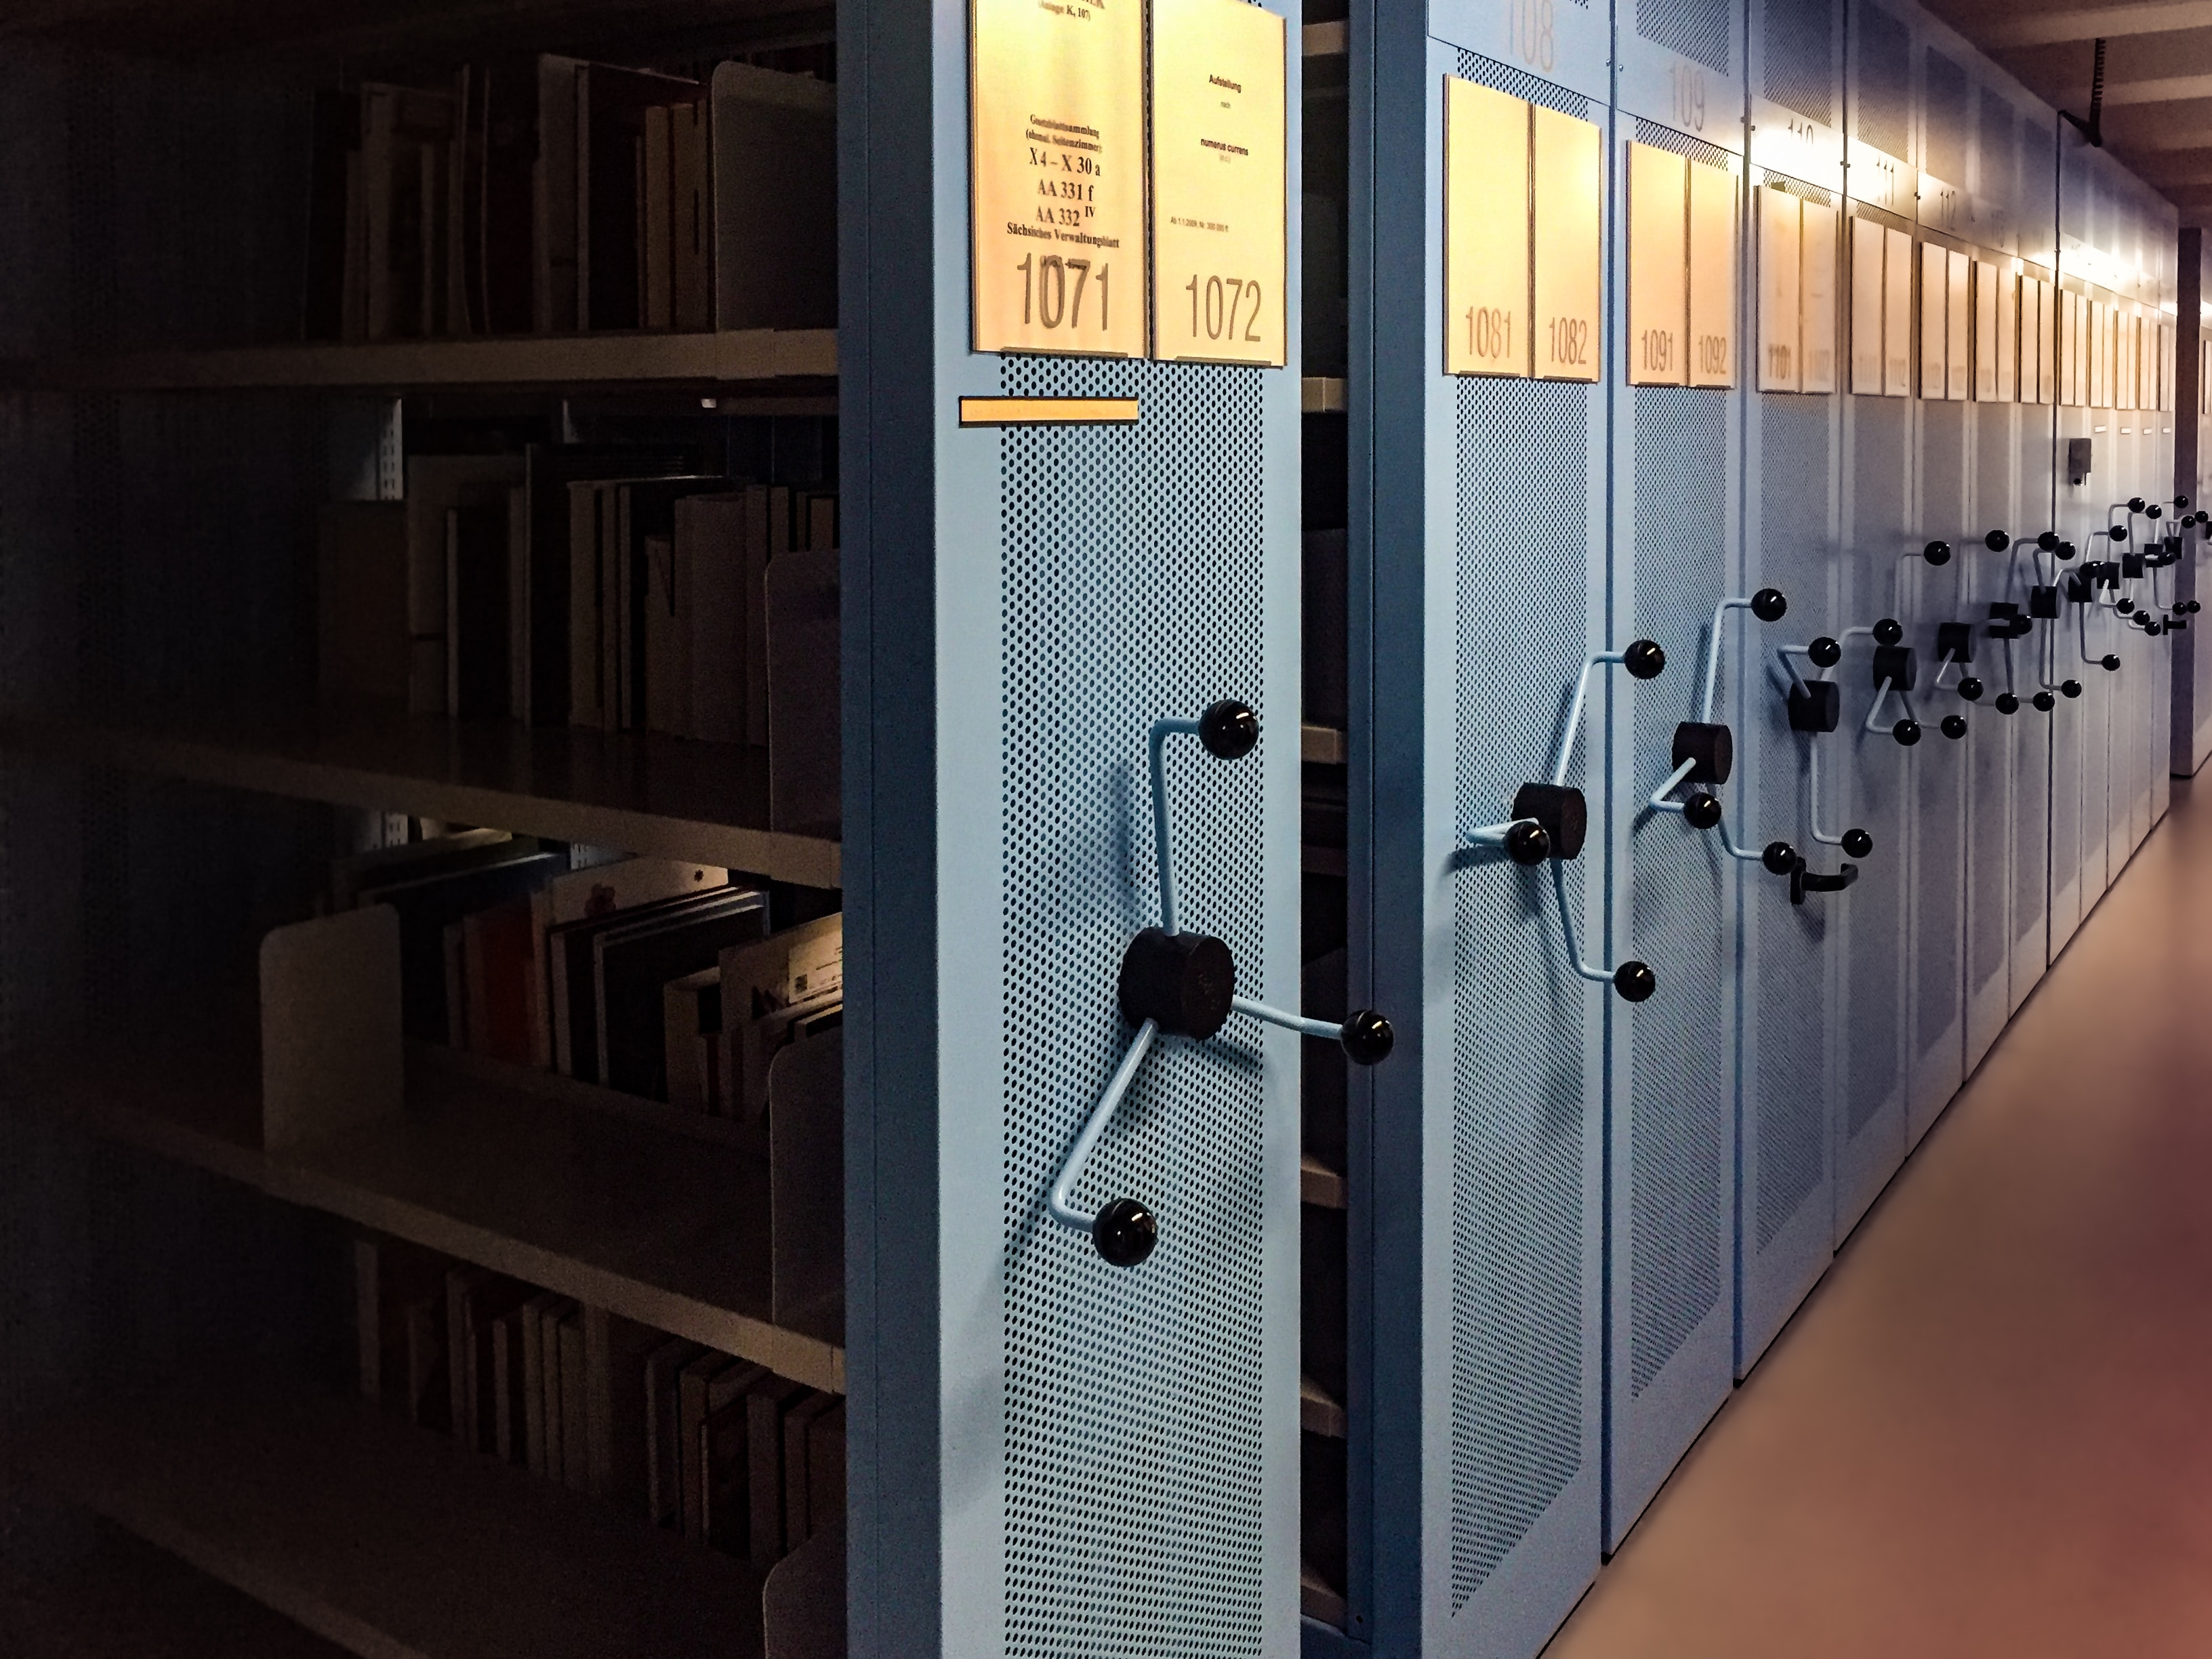
\includegraphics{archive-title-image}}
\advisor{Dr. Simon Kramer}
\coadvisor{Frank Helbling}
%\projectpartner{proj partner}
%\expert{Some expert}
\degreeprogram{Project 1}
\setupSignature{
	N. Dora={
\includegraphics[width=.5\linewidth]{sig_muster}},
	A. Vejseli={
\includegraphics[width=.5\linewidth]{sig_example}},
	K. Wampfler={
\includegraphics[width=.5\linewidth]{sig_example}}
}


%----------------  BFH tile page   -----------------------------------------
\maketitle
%------------ ABSTRACT        ----------------
%\addchap{Abstract}
%The URL-Archiver is a platform-independent Java application which specializes in extracting and archiving URLs from Unicode text or PDF files. It supports archiving on Archive Today and the Wayback Machine, with options to export archived URLs into CSV or the original Bibtex files. The application was developed with a focus on simplicity, modularity and self-explanatory code.

This report details the development process of the URL-Archiver, explaining the implementation strategies, SCRUM methodology and challenges overcome, and concludes with a outlook on potential future enhancements.

%------------ TABLEOFCONTENTS ----------------
\tableofcontents

%------------ List of Tables -------------
\listoftables

%------------ List of Figures ------------
\listoffigures

%------------ List of Listings -----------
%\lstlistoflistings

%------------ START MAIN PART ------------
\mainmatter

\chapter{Introduction}
\section{Initial Situation}
The Internet is constantly evolving, which means that there is no guarantee that a website as it exists today will still exist in a few years' time, let alone contain the same information. While this might not be a concern that the average Internet user has to grapple with, it poses a challenge to the academic demographic, where it becomes crucial to reference sources and potentially integrate links to additional data. If links become inactive, verifying the sources becomes challenging, if not impracticable.

Archiving the existing status of a website is achievable, but it currently necessitates a manual and hence time-intensive operation, which not many people take the time to do. The objective of this project is to devise an automated solution to this predicament that is independent of platforms.

The stakeholders for this solution include:
\begin{itemize}
	\item Legal professionals and researchers who need to preserve web content as evidence or for case study references.
	\item Journalists and media agencies that require archiving web pages for future reporting or fact-checking.
	\item Librarians and archivists tasked with the digital preservation of online materials for historical records.
	\item Content creators and marketers who wish to maintain records of web content for portfolio or audit purposes.
	\item Educators and students who need to collect and cite online resources for academic projects and research.
	\item Organizations and businesses that need to archive their web presence for compliance and record-keeping.
\end{itemize}


\section{Poduct Goal}
The product goal is a platform independent Java application called ``URL-Archiver``.
The application must be Free/Libre and Open Source Software (FLOSS) licensed and fulfil the following functionalities:
\begin{enumerate}
    \item The software should be CLI\footnote{Command Line Interface}-based and offer a clear command line.
    \item The software should allow the user to input a path, which can be a folder or any Unicode text file.
    \item The software examines the contents of a file or folder to extract any web URLs using a standard regular expression or similar method.
    \item If desired, URLs can be automatically opened in a web browser.
    \item The extracted URLs are archived on archive.today and/or web.archive.org (known as The Wayback Machine) as per the user's preference.
    \item The software outputs the resulting archive URLs to the user.
    \item The software generates a CSV file containing the original URL and the archived Version of the URL.
    \item Optionally, the archived Versions are written back into the provided .bib file.
\end{enumerate}
The product goal is achieved if the software covers all the functionality listed above.
Furthermore, the code should be minimalistic, modular, and self-explaining.
In addition to the code, it is essential that the following documents are provided:
\begin{itemize}
    \item User manual
    \item Installation instructions (including installation script)
    \item Software documentation
\end{itemize}

\section{Priorities}
The following priorities are listed in order of importance:
\begin{enumerate}
    \item \textbf{Functionality}: The primary priority is the accurate extraction and archiving of URLs. The software should reliably identify URLs in varied file types and ensure their successful archiving on \href{https://archive.ph}{https://archive.ph} or \href{https://web.archive.org/save/}{Wayback Machine}.
    \item \textbf{Usability}: Given the diverse potential user base, the program should be platform-independent and possess a user-friendly interface. While the underlying mechanisms may be complex, the user experience should be seamless and intuitive.
    \item \textbf{Code Quality}: Emphasis should be placed on writing clean, minimal, and modular code. This not only aids in potential future enhancements but also in debugging and troubleshooting.
    \item \textbf{Documentation}: As with any software project, proper documentation is paramount. The project report should be concise, adhering to the principle of being ``maximally informative, minimally long,`` ensuring clarity of information without overwhelming the reader.
    \item \textbf{Integration with Existing File Types}: The ability to seamlessly insert archived URLs into .BIB files is a priority, given the potential academic applications of the software.
\end{enumerate}

\chapter{Scrum Implementation}
\subsection{Allocation of roles}
In this chapter, the Scrum roles (Product Owner, Scrum Master, Developer) and additional roles such as Customer, Stakeholder, etc. are defined.


\subsection{Scrum roles}
We have decided to structure our Scrum team in the following manner:
\begin{table}[ht]
    \centering
    \begin{bfhTabular}{lll}
        \textbf{Role} & \textbf{Person}\\\hline
        Product Owner & Nicolin Dora\\\hline
        Scrum Master  & Abidin Vejseli\\\hline
        Developer     & Nicolin Dora, Abidin Vejseli, Kilian Wampfler\\\hline
    \end{bfhTabular}
    \caption{Scrum Roles}
    \label{tab:tab1}
\end{table}

Nicolin took on the role of Product Owner as he had concrete ideas and visions for the product at the start of the project.
Additionally, he took on this role because he wanted to deal with the subjects surrounding the product backlog.

Abidin took on the role of the Scrum Master as he has the most experience with the agile way of working.
He has already had the opportunity to perform this role professionally on several smaller projects in the past.

Kilian took on the role of a Developer, as he is an active programmer in his job and has already gained some experience with Scrum.
Therefore, self-organization is not a foreign concept to him.

Besides Kilian, all the other members of the group were also assigned the role of Developer, as otherwise the project would not have been feasible in the given time. This is due to the fact that we all work alongside the university.


\subsection{Additional roles}
In addition to the Scrum roles, we have assigned the following roles to our specialist lecturer and PM-coach.
\begin{table}[ht]
    \centering
    \begin{bfhTabular}{lll}
        \textbf{Role} & \textbf{Person}\\\hline
        Stakeholder   & Dr. Simon Kramer\\\hline
        Customer      & Dr. Simon Kramer\\\hline
        PM-Advisor    & Frank Helbling\\\hline
    \end{bfhTabular}
    \caption{Additional Scrum Roles}
    \label{tab:tab2}
\end{table}


\subsection{Sprint Goals}
We have defined the goals of our past and current sprints in the best possible way according to the SMART\footnote{\href{https://www.atlassian.com/blog/productivity/how-to-write-smart-goals}{Atlassian blogpost: "How to write smart goals"}} criteria. The goals of our sprints are listed below:

\paragraph{Sprint 1}
Implement input handler for files (any unicode file e.g. .bib, .txt, .html and .pdf) and basic user guidance (Menu, Error messages).

\paragraph{Sprint 2}
Implement a function to scan a provided text in order to identify and extract any URLs contained within it and upgrade our current console-based interface to enable users to easily open any extracted URL using their default web browser.

\paragraph{Sprint 3}
Develop and implement a fully automated URL submission system that integrates with the Wayback Machine and Archive Today to ensure at least a 98% success rate in URL archiving.

\paragraph{Sprint 4}
Enhance the system's stability and usability by resolving identified Selenium bugs across Linux, macOS, and Edge browsers, documenting the sprint process and licenses, conducting a thorough code review, and establishing a new configuration management file, aiming for zero critical bugs at sprint closure and readying the system for seamless URL archiving integration in subsequent sprints.

\paragraph{Sprint 5}
Complete application refactoring for asynchronous archiving and .BIB file URL integration, ensuring no critical bugs and preparing for seamless future enhancements.

\paragraph{Sprint 6}
Deliver a finalized application design, improved code quality, and complete documentation, with all components ready for review.

\clearpage

\subsection{Requirements}
In this chapter, we present our product and sprint backlogs, structured according to Scrum.

\subsubsection{Product Backlog}
Our product backlog consists of user stories and epics created by our Product Owner.
The user stories are prioritised and represent a set of initial requirements that must be met to achieve our product goal. The product backlog is maintained in Jira.
\begin{figure}[h!]
    \centering
    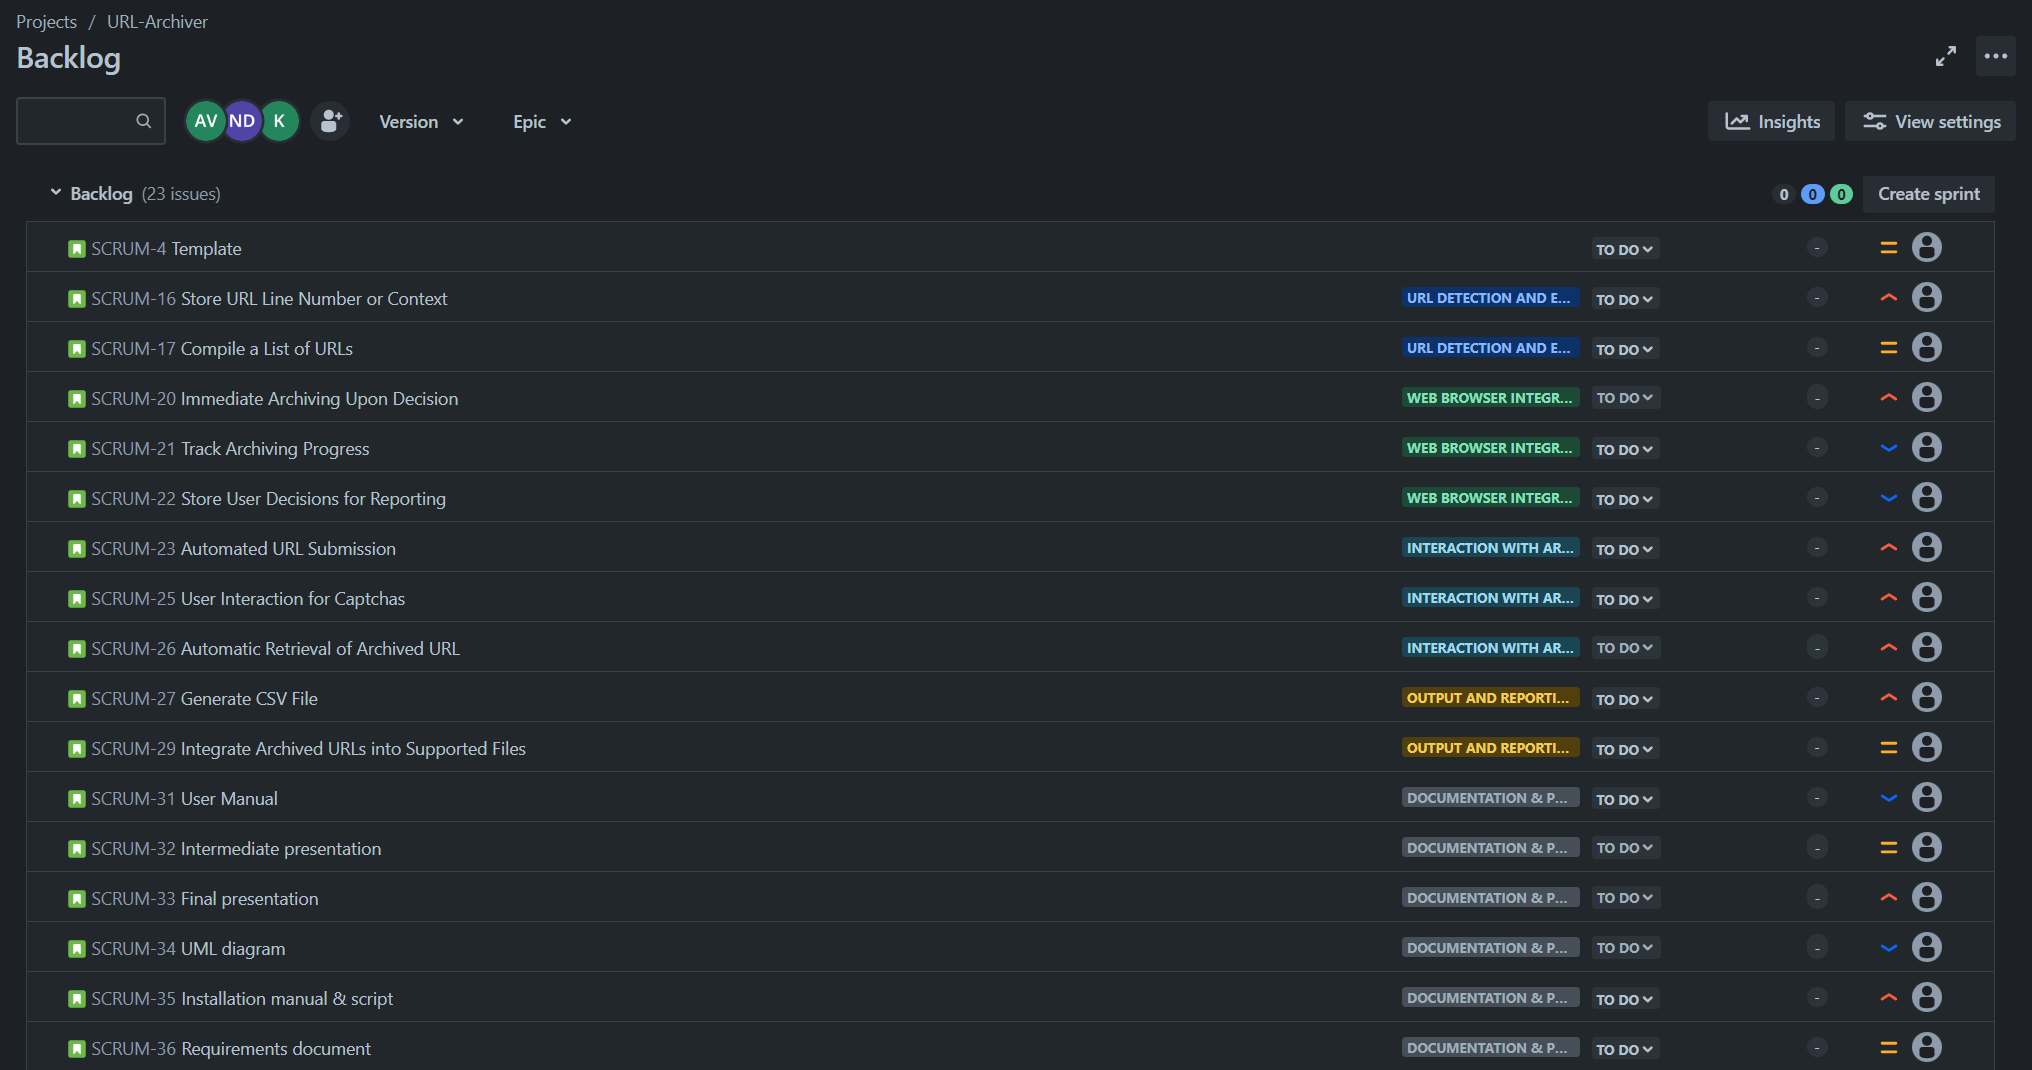
\includegraphics[width=1\textwidth]{pictures/backlog}
    \caption{Product Backlog}
    \label{fig:backlog}
\end{figure}

The prioritisation of user stories in the backlog is based on the business value field, which has a value between one and ten.
The business value is a vague estimate of how much value the individual user story has to the business, or in our case, to our stakeholders.
We endeavour to estimate the business value based on the expected importance of the function to the stakeholder.
The following priorities are possible:
\begin{itemize}
    \item Highest
    \item High
    \item Medium
    \item Low
    \item Lowest
\end{itemize}

\subsubsection{Sprint Backlogs}
Below we describe our recent and current sprints.
During the sprint planning we fill the respective sprint backlog with user stories that serve the sprint goal.
A user story must satisfy our Definition of Ready before it can be included in the sprint.
In addition, the stories must be estimated and the total number of story points must not exceed our defined velocity.

\paragraph{Sprint 1}
Below is a screenshot of our board from the first sprint with the corresponding sprint goal.
\begin{figure}[h!]
    \centering
    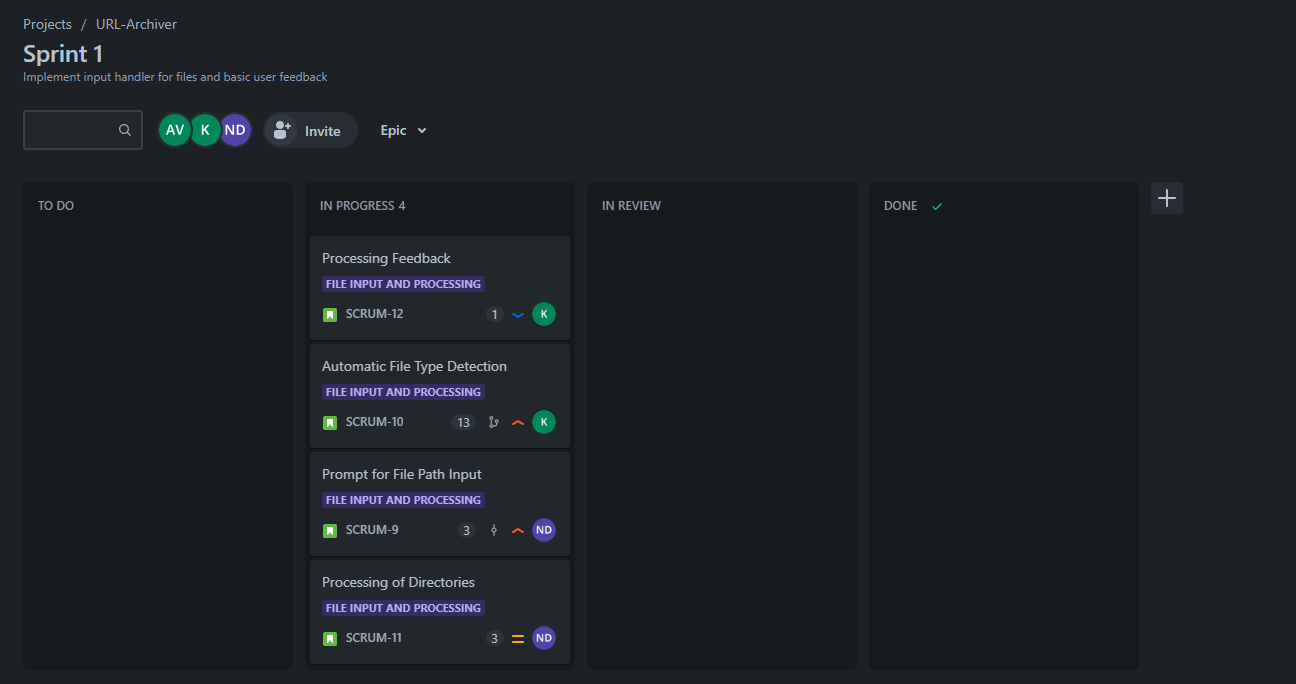
\includegraphics[width=1\textwidth]{pictures/backlog_sprint_1}
    \caption{Sprint 1 Backlog}
    \label{fig:backlog_sprint_1}
\end{figure}

The user stories from the first sprint are shown below. The stories have been estimated and prioritised.

\begin{figure}[h!]
    \centering
    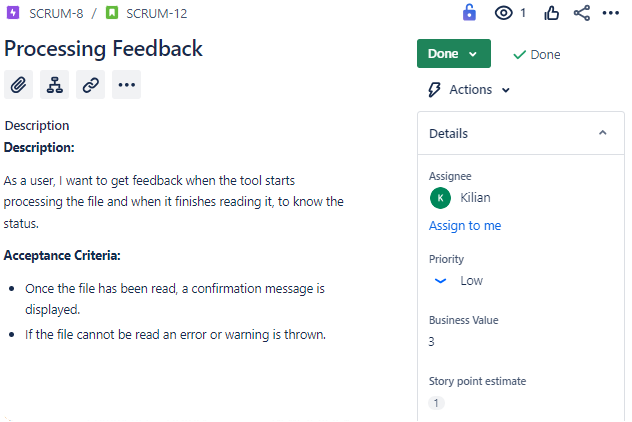
\includegraphics[width=1\textwidth]{pictures/Scrum/Sprint 1/UserStory_4}
    \caption{User Story Detail for "Processing Feedback"}
    \label{fig:sprint_1_userstory_1}
\end{figure}
\begin{figure}[h!]
    \centering
    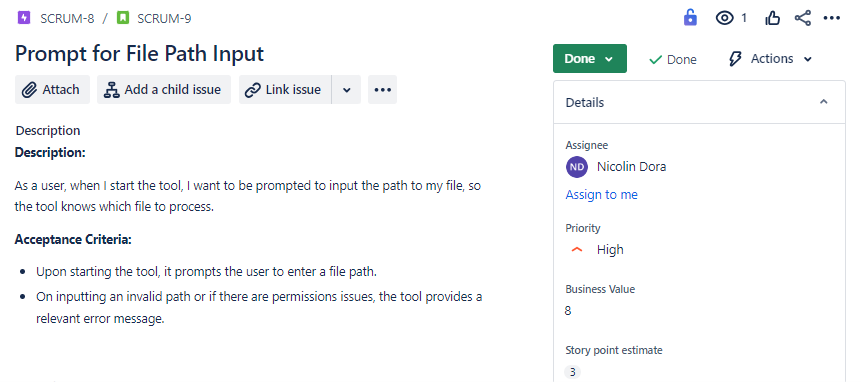
\includegraphics[width=1\textwidth]{pictures/Scrum/Sprint 1/UserStory_1}
    \caption{User Story Detail for "Prompt for file path input"}
    \label{fig:sprint_1_userstory_2}
\end{figure}
\begin{figure}[h!]
    \centering
    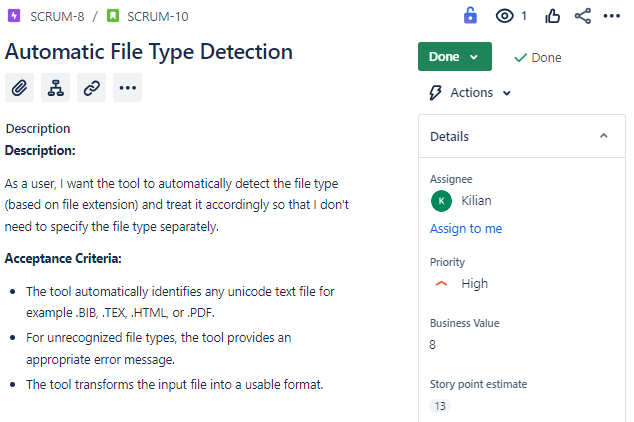
\includegraphics[width=1\textwidth]{pictures/Scrum/Sprint 1/UserStory_2}
    \caption{User Story Detail for "Automatic File Type Detection"}
    \label{fig:sprint_1_userstory_3}
\end{figure}
\begin{figure}[h!]
    \centering
    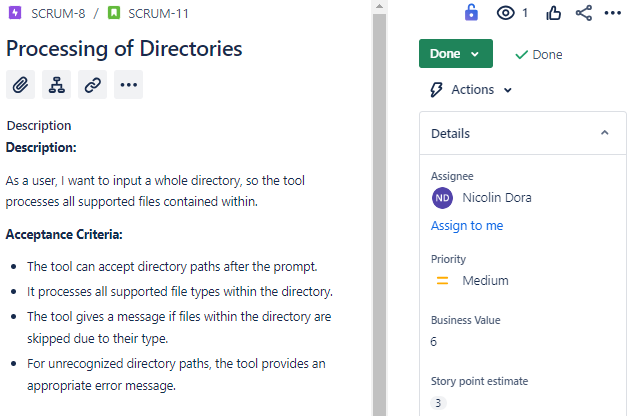
\includegraphics[width=1\textwidth]{pictures/Scrum/Sprint 1/UserStory_3}
    \caption{User Story Detail for "Processing of Directories"}
    \label{fig:sprint_1_userstory_4}
\end{figure}
\clearpage

In the first sprint, the burn down chart looks like this:
\begin{figure}[h!]
    \centering
    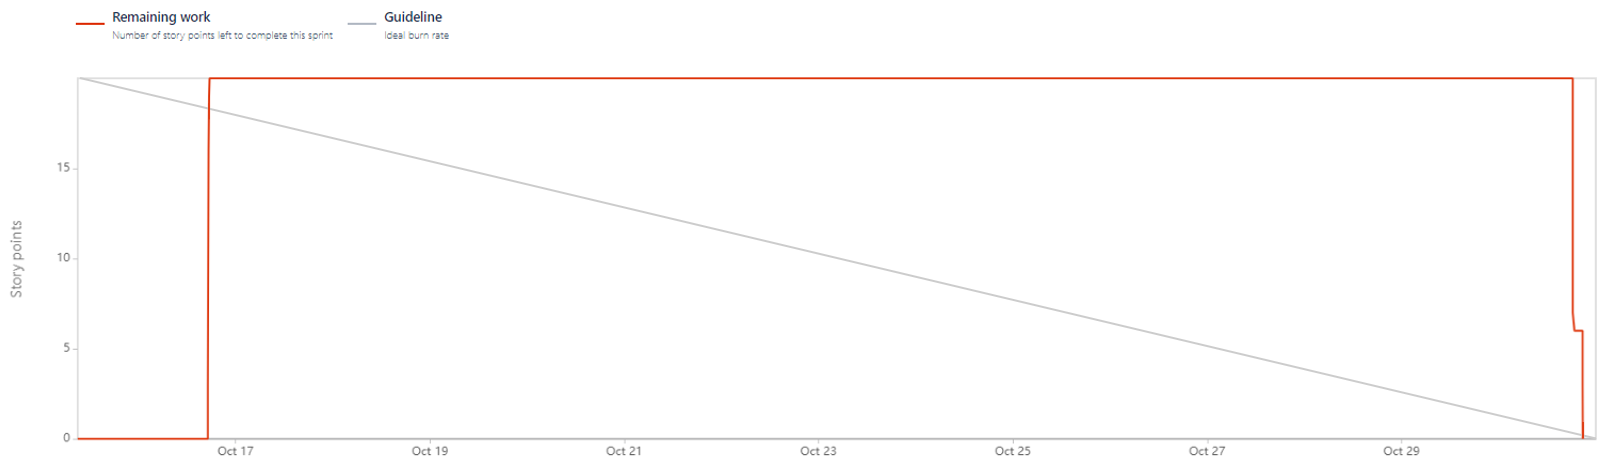
\includegraphics[width=1\textwidth]{pictures/Scrum/Sprint 1/sprint1_burndownchart}
    \caption{Sprint 1 Burn Up Chart}
    \label{fig:sprint_1_bunrdown_chart}
\end{figure}

The reason for this is that we did not create tasks for our user stories as they were small enough.
Furthermore, a code review for corresponding user stories could only be conducted towards the end of the sprint, resulting in the finalisation of user stories at that point.
\clearpage

\paragraph{Sprint 2}
Below is a screenshot of our board from the second sprint with the corresponding sprint goal.
\begin{figure}[h!]
    \centering
    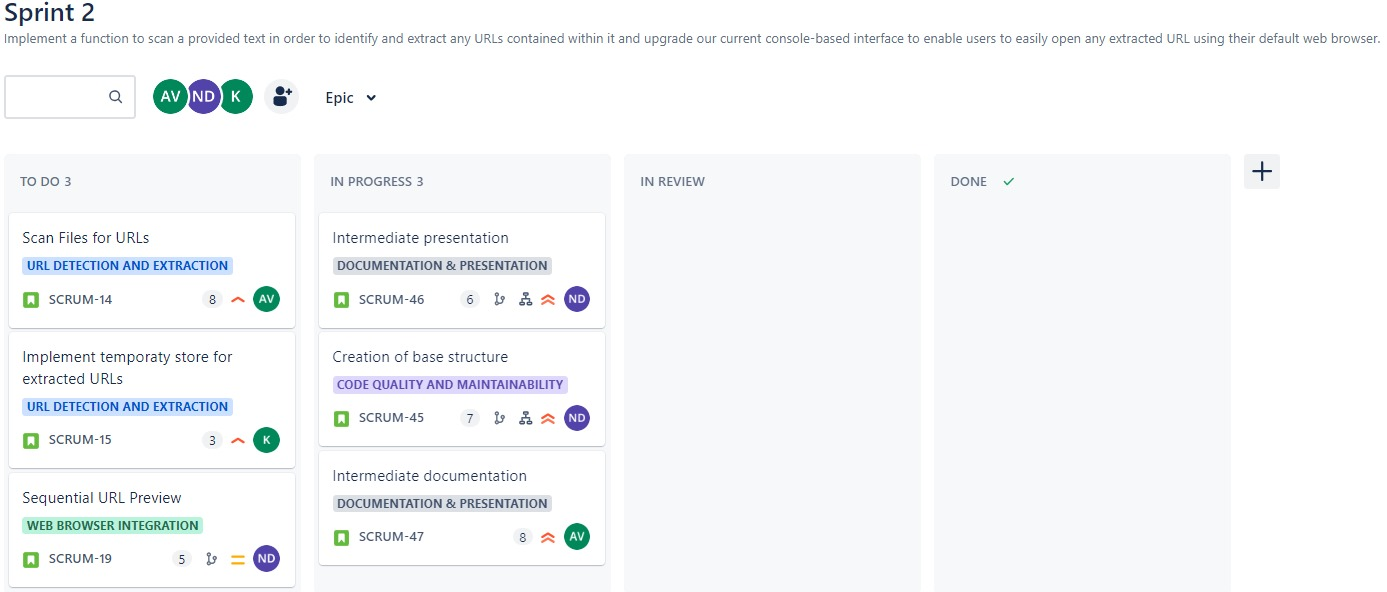
\includegraphics[width=1\textwidth]{pictures/Scrum/Sprint 2/Sprint2_Backlog}
    \caption{Sprint 2 Backlog}
    \label{fig:sprint_2_backlog}
\end{figure}

The user stories from the second sprint are shown below. The stories have been estimated and prioritised.
\begin{figure}[h!]
    \centering
    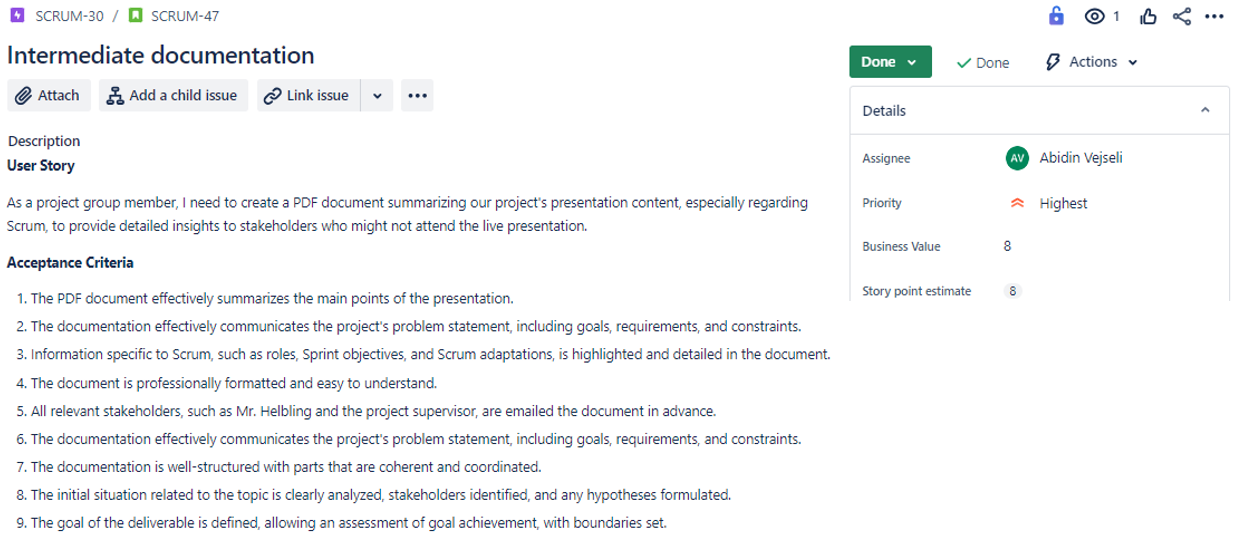
\includegraphics[width=1\textwidth]{pictures/Scrum/Sprint 2/UserStory_13}
    \caption{User Story Detail for "Intermediate Documentation"}
    \label{fig:sprint_2_userstory_1}
\end{figure}
\begin{figure}[h!]
    \centering
    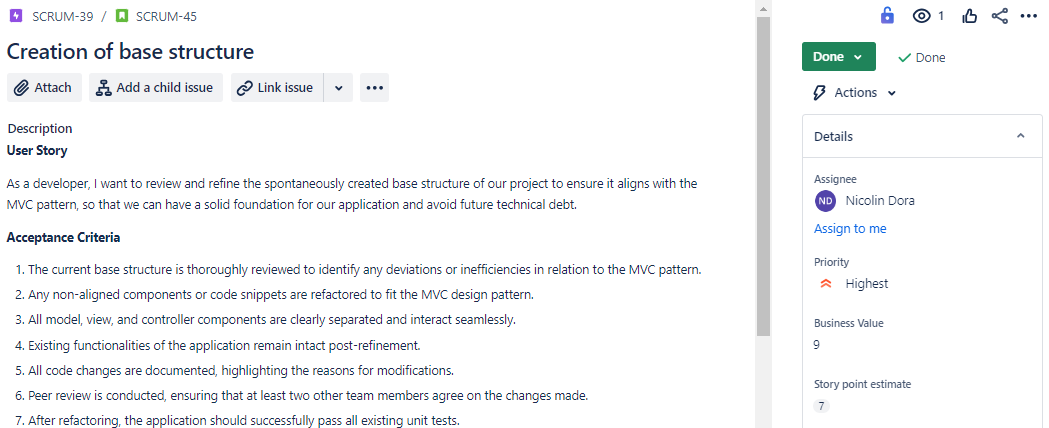
\includegraphics[width=1\textwidth]{pictures/Scrum/Sprint 2/UserStory_11}
    \caption{User Story Detail for "Creation of Base Structure"}
    \label{fig:sprint_2_userstory_2}
\end{figure}
\begin{figure}[h!]
    \centering
    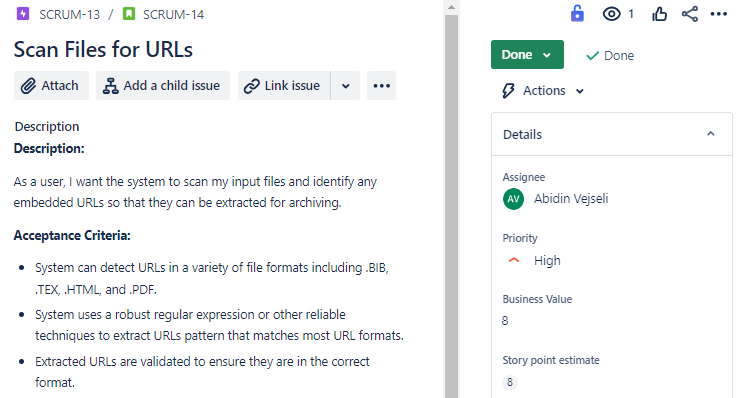
\includegraphics[width=1\textwidth]{pictures/Scrum/Sprint 2/UserStory_5}
    \caption{User Story Detail for "Scan Files for URLs"}
    \label{fig:sprint_2_userstory_3}
\end{figure}
\begin{figure}[h!]
    \centering
    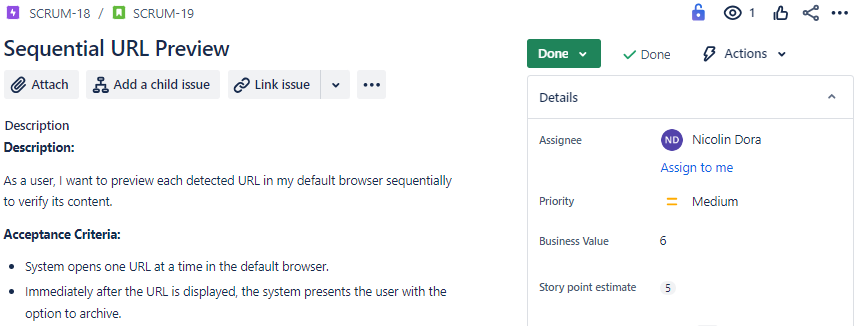
\includegraphics[width=1\textwidth]{pictures/Scrum/Sprint 2/UserStory_7}
    \caption{User Story Detail for "Sequential URL Preview"}
    \label{fig:sprint_2_userstory_4}
\end{figure}
\begin{figure}[h!]
    \centering
    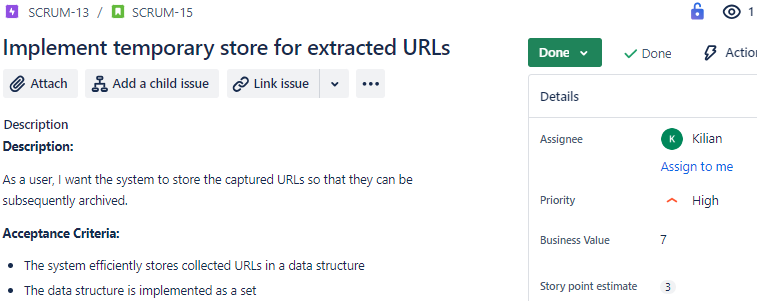
\includegraphics[width=1\textwidth]{pictures/Scrum/Sprint 2/UserStory_6}
    \caption{User Story Detail for "Implement temporary store for extracted URLs"}
    \label{fig:sprint_2_userstory_5}
\end{figure}
\begin{figure}[h!]
    \centering
    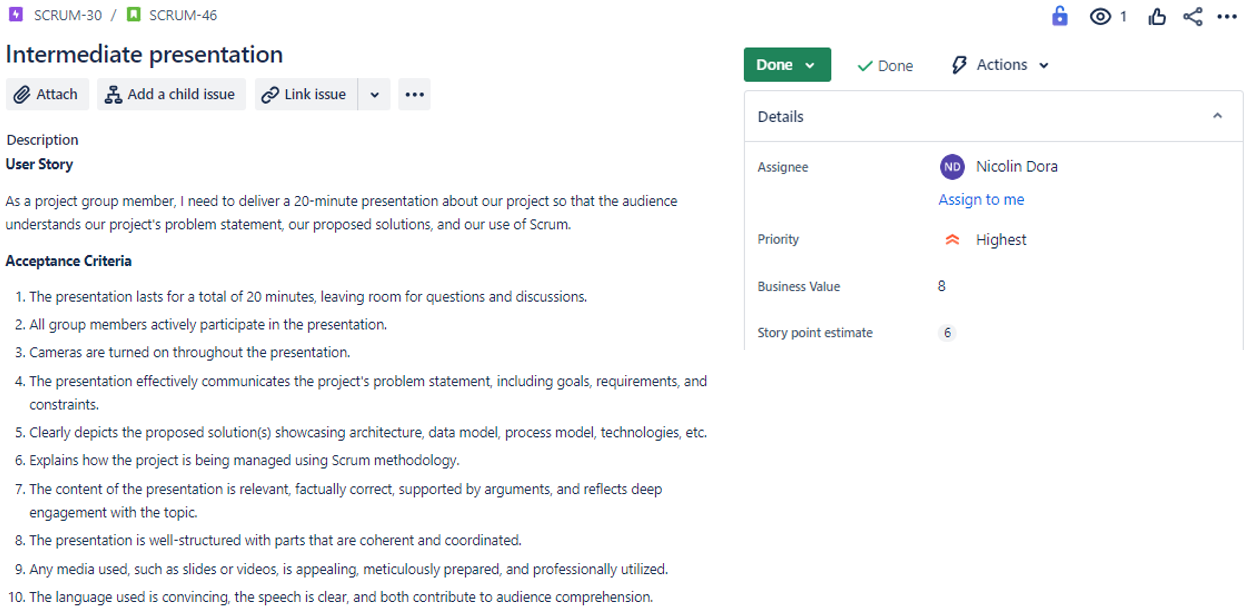
\includegraphics[width=1\textwidth]{pictures/Scrum/Sprint 2/UserStory_12}
    \caption{User Story Detail for "Intermediate presentation"}
    \label{fig:sprint_2_userstory_6}
\end{figure}
\clearpage

In the second sprint, the burn down chart looks like this:
\begin{figure}[h!]
    \centering
    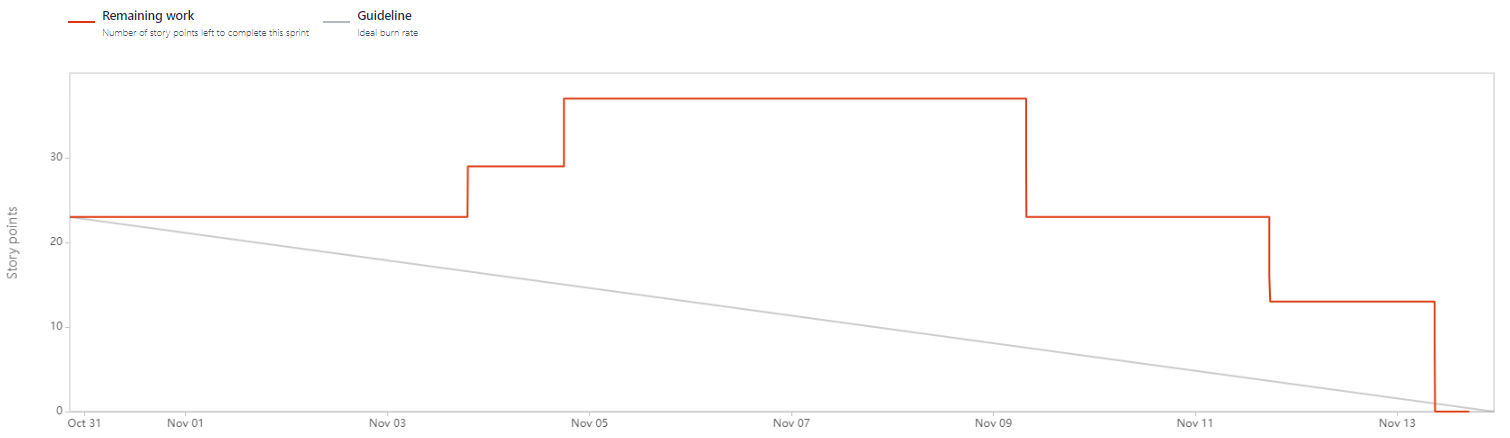
\includegraphics[width=1\textwidth]{pictures/Scrum/Sprint 2/Sprint2_burndownchart}
    \caption{Sprint 2 Burn Down Chart}
    \label{fig:sprint_2_bunrdown_chart}
\end{figure}

Compared to the initial sprint, our workload significantly increased, and we introduced new user stories after the sprint began.
Despite these additions, we maintained a strong pace and seamlessly managed the extra tasks that arose from the intermediate presentation and documentation requirements.
\clearpage


\paragraph{Sprint 3}
Below is a screenshot of our board from the third sprint with the corresponding sprint goal.
\begin{figure}[h!]
    \centering
    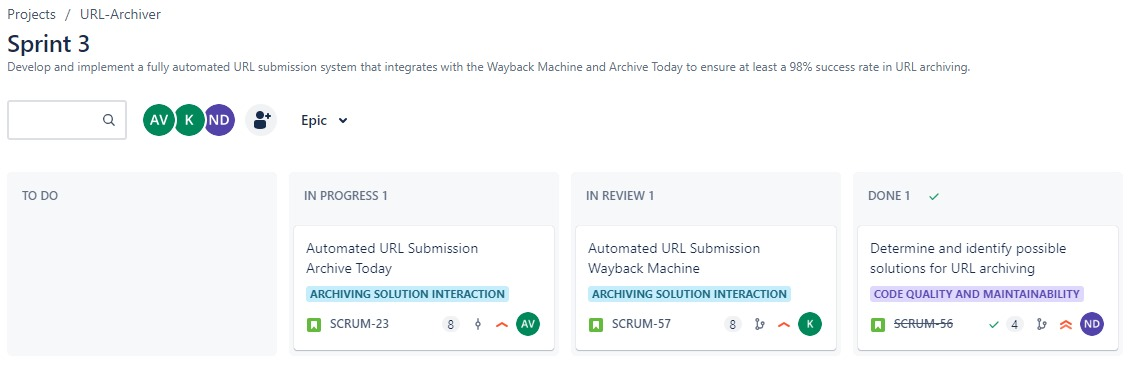
\includegraphics[width=1\textwidth]{pictures/Scrum/Sprint 3/Sprint3_Backlog}
    \caption{Sprint 3 Backlog}
    \label{fig:sprint_3_backlog}
\end{figure}

The user stories from the third sprint are shown below. The stories have been estimated and prioritised.
\begin{figure}[h!]
    \centering
    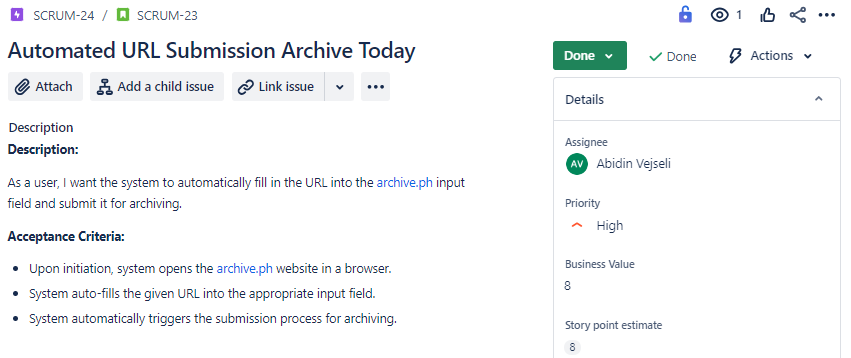
\includegraphics[width=1\textwidth]{pictures/Scrum/Sprint 3/UserStory_8}
    \caption{User Story Detail for "Intermediate Documentation"}
    \label{fig:sprint_3_userstory_1}
\end{figure}
\begin{figure}[h!]
    \centering
    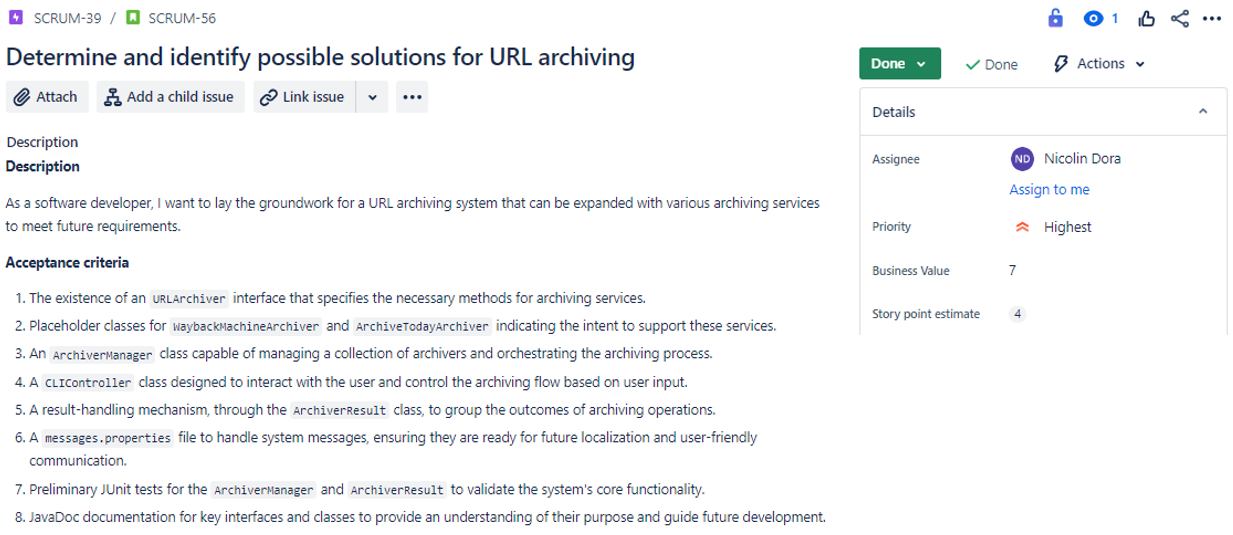
\includegraphics[width=1\textwidth]{pictures/Scrum/Sprint 3/UserStory_14}
    \caption{User Story Detail for "Creation of Base Structure"}
    \label{fig:sprint_3_userstory_2}
\end{figure}
\begin{figure}[h!]
    \centering
    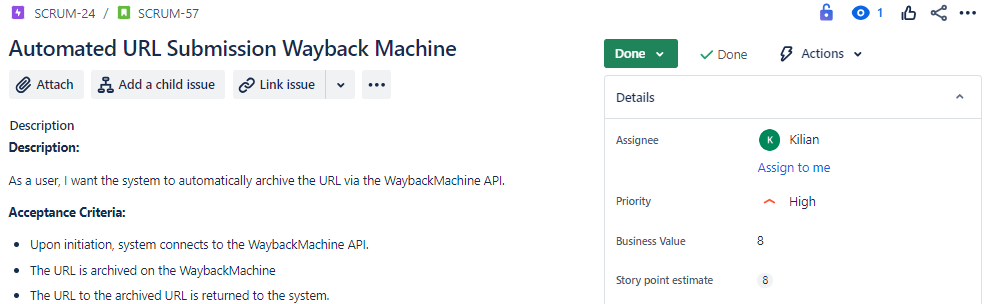
\includegraphics[width=1\textwidth]{pictures/Scrum/Sprint 3/UserStory_15}
    \caption{User Story Detail for "Scan Files for URLs"}
    \label{fig:sprint_3_userstory_3}
\end{figure}

In the third sprint, the burn down chart looks like this:
\begin{figure}[h!]
    \centering
    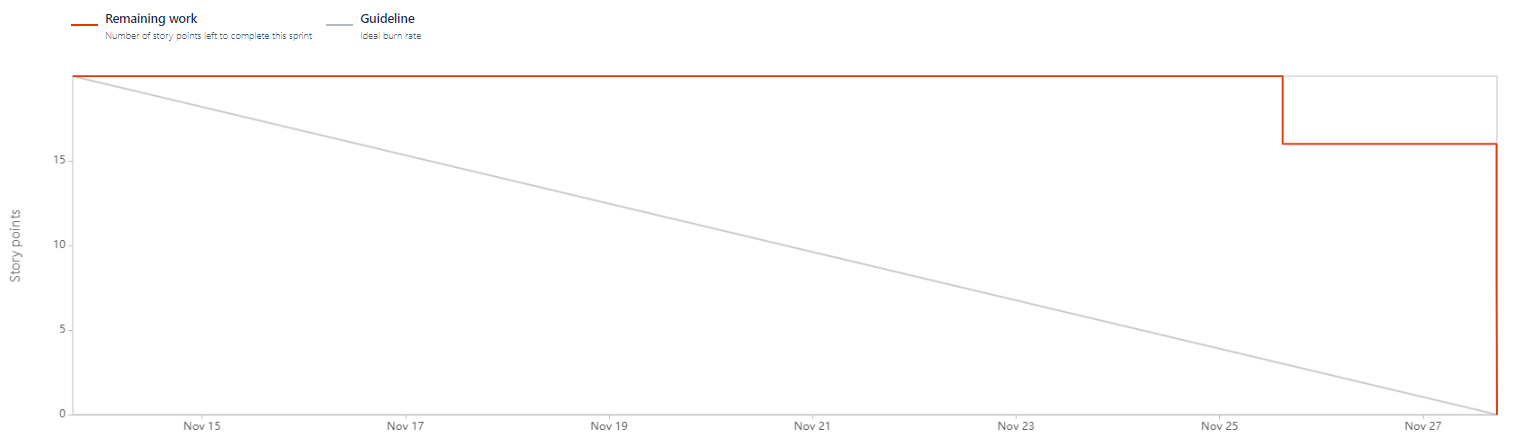
\includegraphics[width=1\textwidth]{pictures/Scrum/Sprint 3/Sprint3_burndownchart}
    \caption{Sprint 3 Burn Down Chart}
    \label{fig:sprint_3_bunrdown_chart}
\end{figure}

During the third sprint, our progress on user stories was limited to the completion of only three due to the 'special week 3'.
This meant that these stories had to be completed in the second half of the sprint due to the heavy workload of this special week.
The impact of this adaptation to our sprint schedule due to 'special week 3' is reflected in the trends seen in our burndown chart.
\clearpage

\paragraph{Sprint 4}
Below is a screenshot of our board from the forth sprint.
\begin{figure}[h!]
    \centering
    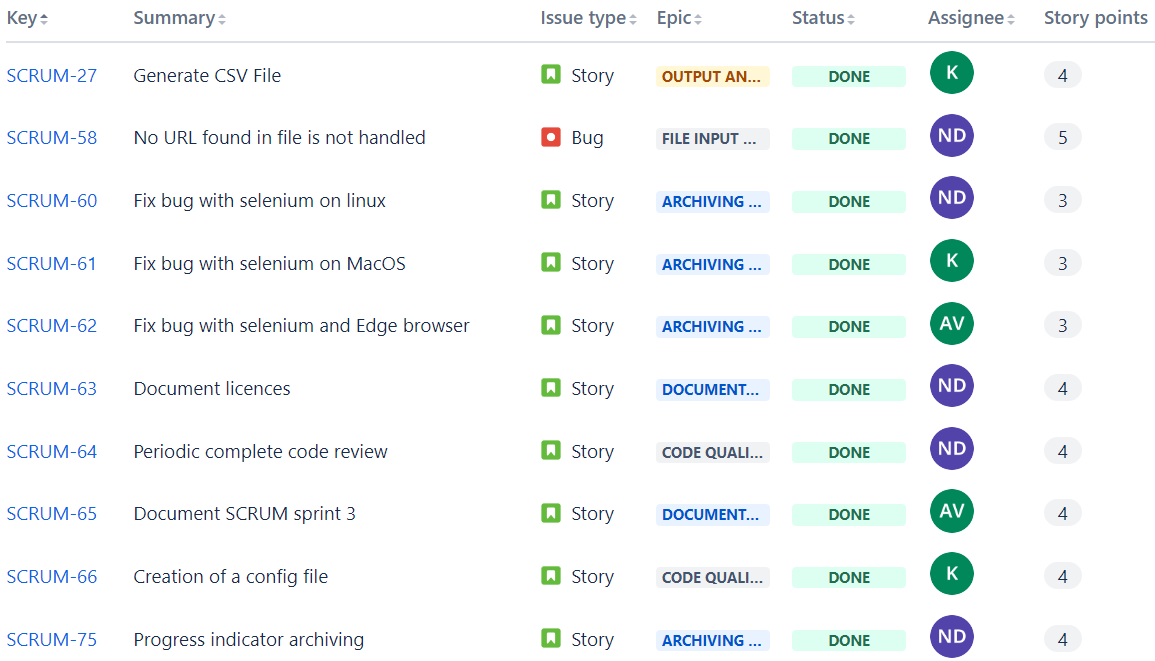
\includegraphics[width=1\textwidth]{pictures/Scrum/Sprint 4/Sprint4_Backlog}
    \caption{Sprint 4 Backlog}
    \label{fig:sprint_4_backlog}
\end{figure}

The user stories from the forth sprint are shown below. The stories have been estimated and prioritised.
\begin{figure}[h!]
    \centering
    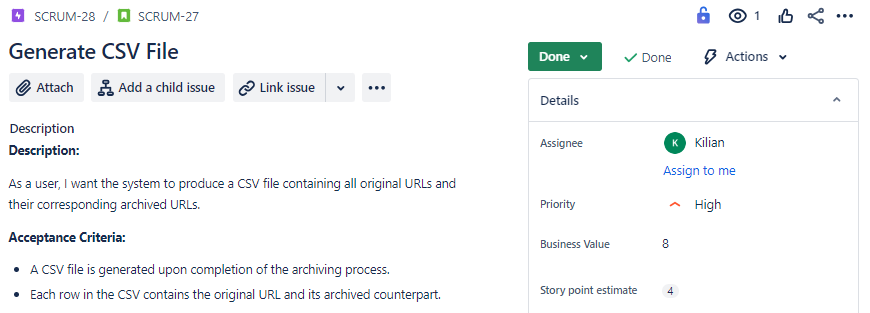
\includegraphics[width=1\textwidth]{pictures/Scrum/Sprint 4/UserStory_9}
    \caption{User Story Detail for "Generate CSV File"}
    \label{fig:sprint_4_userstory_1}
\end{figure}
\begin{figure}[h!]
    \centering
    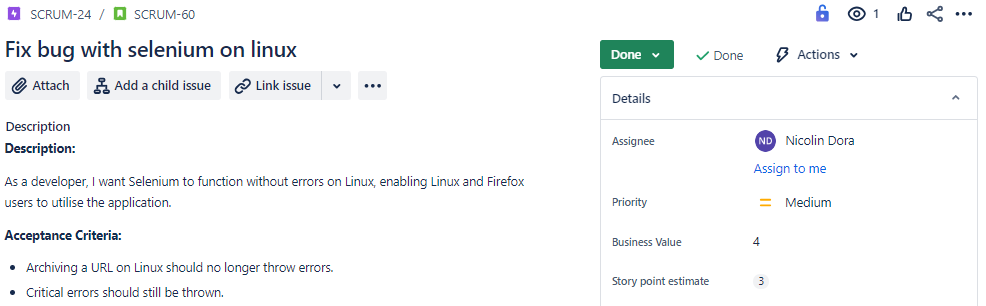
\includegraphics[width=1\textwidth]{pictures/Scrum/Sprint 4/UserStory_16}
    \caption{User Story Detail for "Fix bug with selenium on linux"}
    \label{fig:sprint_4_userstory_2}
\end{figure}
\begin{figure}[h!]
    \centering
    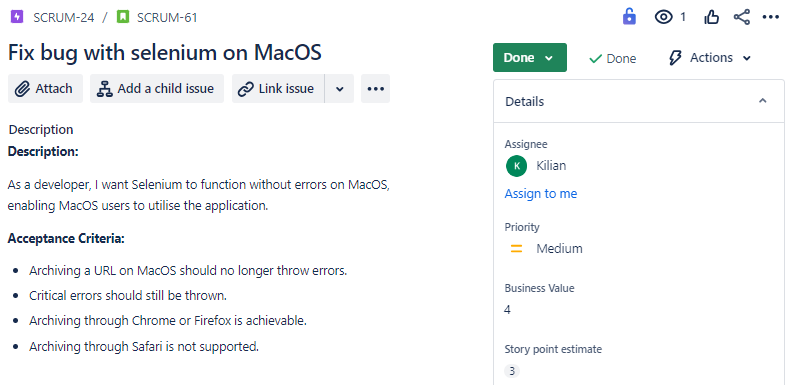
\includegraphics[width=1\textwidth]{pictures/Scrum/Sprint 4/UserStory_17}
    \caption{User Story Detail for "Fix bug with selenium on MacOS"}
    \label{fig:sprint_4_userstory_3}
\end{figure}
\begin{figure}[h!]
    \centering
    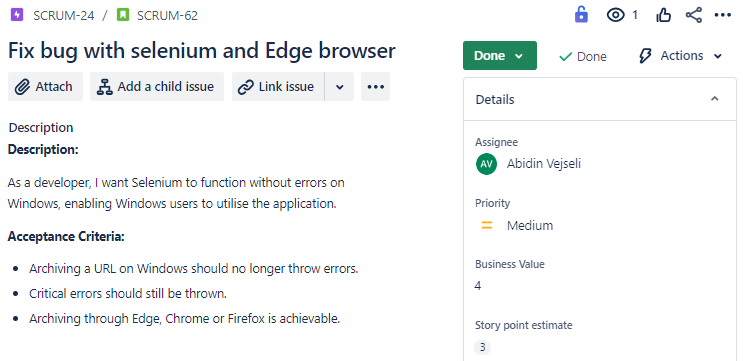
\includegraphics[width=1\textwidth]{pictures/Scrum/Sprint 4/UserStory_18}
    \caption{User Story Detail for "Fix bug With selenium and Edge browser"}
    \label{fig:sprint_4_userstory_4}
\end{figure}
\begin{figure}[h!]
    \centering
    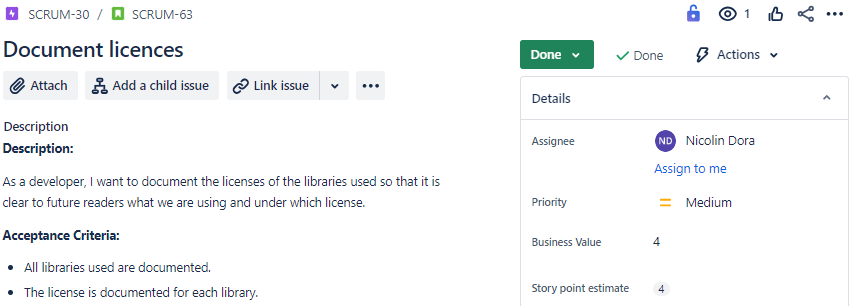
\includegraphics[width=1\textwidth]{pictures/Scrum/Sprint 4/UserStory_19}
    \caption{User Story Detail for "Document licences"}
    \label{fig:sprint_4_userstory_5}
\end{figure}
\begin{figure}[h!]
    \centering
    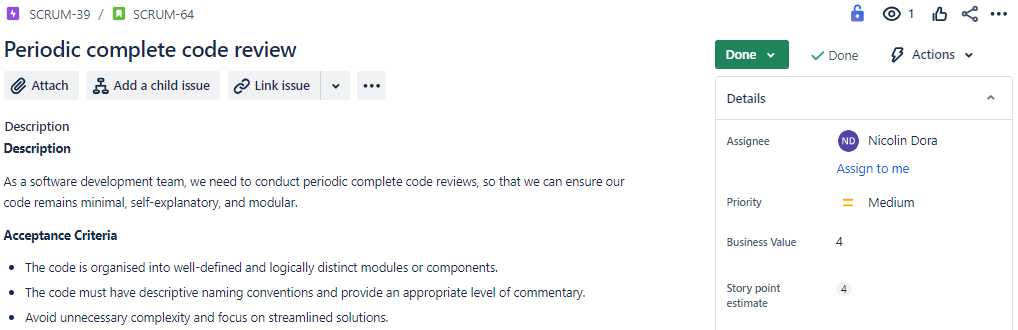
\includegraphics[width=1\textwidth]{pictures/Scrum/Sprint 4/UserStory_20}
    \caption{User Story Detail for "Periodic complete code review"}
    \label{fig:sprint_4_userstory_6}
\end{figure}
\begin{figure}[h!]
    \centering
    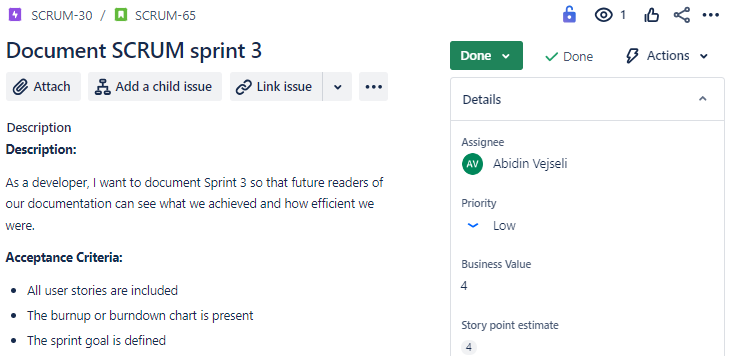
\includegraphics[width=1\textwidth]{pictures/Scrum/Sprint 4/UserStory_21}
    \caption{User Story Detail for "Document SCRUM sprint 3"}
    \label{fig:sprint_4_userstory_7}
\end{figure}
\begin{figure}[h!]
    \centering
    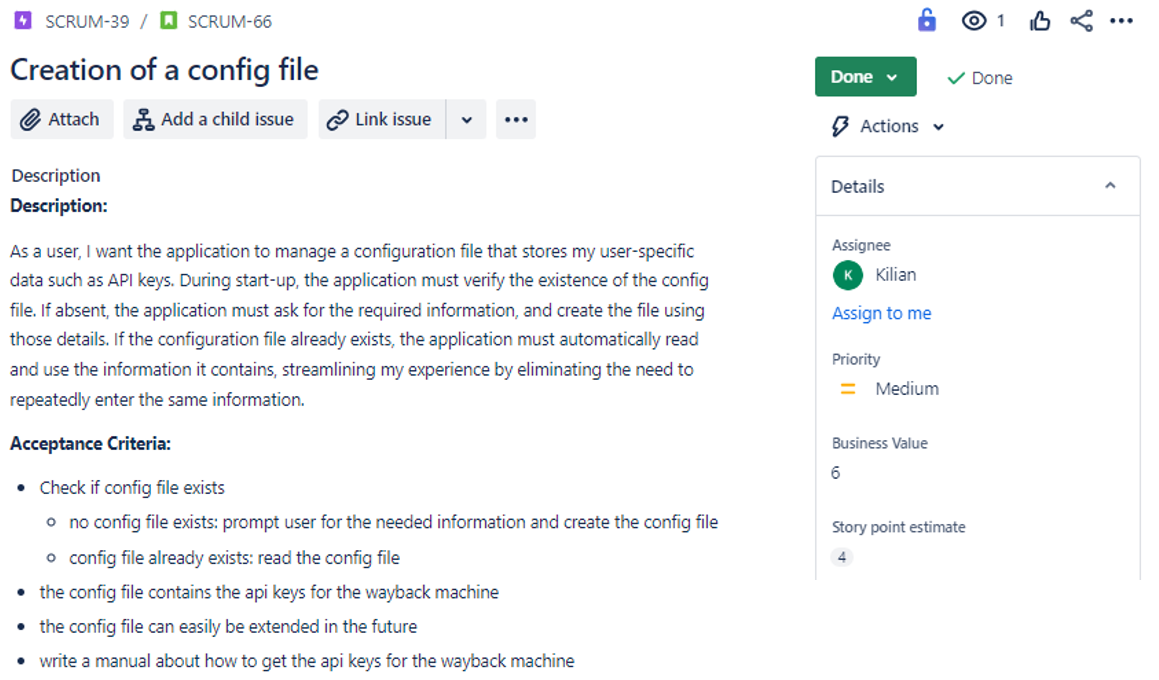
\includegraphics[width=1\textwidth]{pictures/Scrum/Sprint 4/UserStory_22}
    \caption{User Story Detail for "Creation of a config file"}
    \label{fig:sprint_4_userstory_8}
\end{figure}
\begin{figure}[h!]
    \centering
    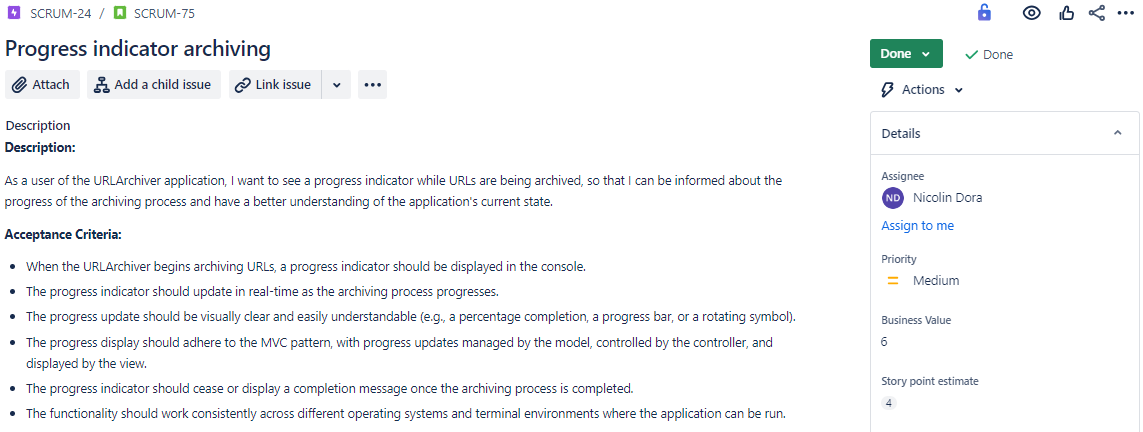
\includegraphics[width=1\textwidth]{pictures/Scrum/Sprint 4/UserStory_24}
    \caption{User Story Detail for "Progress indicator archiving"}
    \label{fig:sprint_4_userstory_9}
\end{figure}
\begin{figure}[h!]
    \centering
    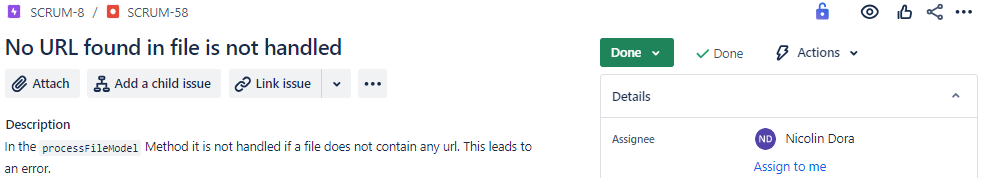
\includegraphics[width=1\textwidth]{pictures/Scrum/Sprint 4/Bug_1}
    \caption{Bug Detail for "No URL found in file is not handled"}
    \label{fig:sprint_4_bug_1}
\end{figure}


In the forth sprint, the burn down chart looks like this:
\begin{figure}[h!]
    \centering
    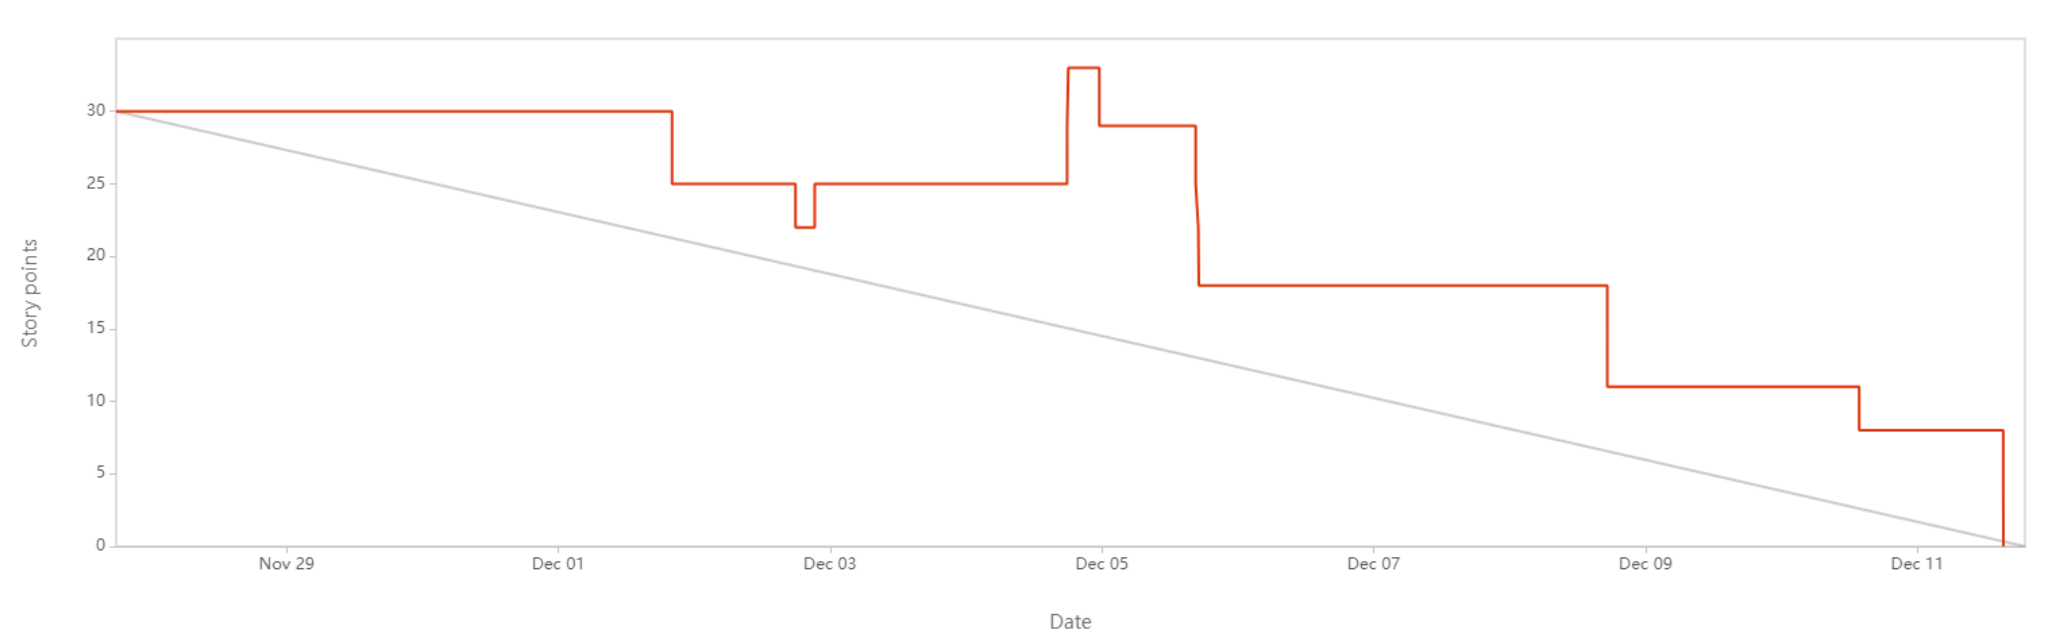
\includegraphics[width=1\textwidth]{pictures/Scrum/Sprint 4/Sprint4_Burndownchart}
    \caption{Sprint 4 Burn Down Chart}
    \label{fig:sprint_4_bunrdown_chart}
\end{figure}

Compared to the previous sprint, we were more efficient and successfully accommodated additional user stories that were initiated after the sprint began.
The completion of all allocated user stories within the sprint timeframe demonstrates our solid teamwork and sprint management capabilities.
\clearpage


\paragraph{Sprint 5}
Below is a screenshot of our board from the fifth sprint.
\begin{figure}[h!]
    \centering
    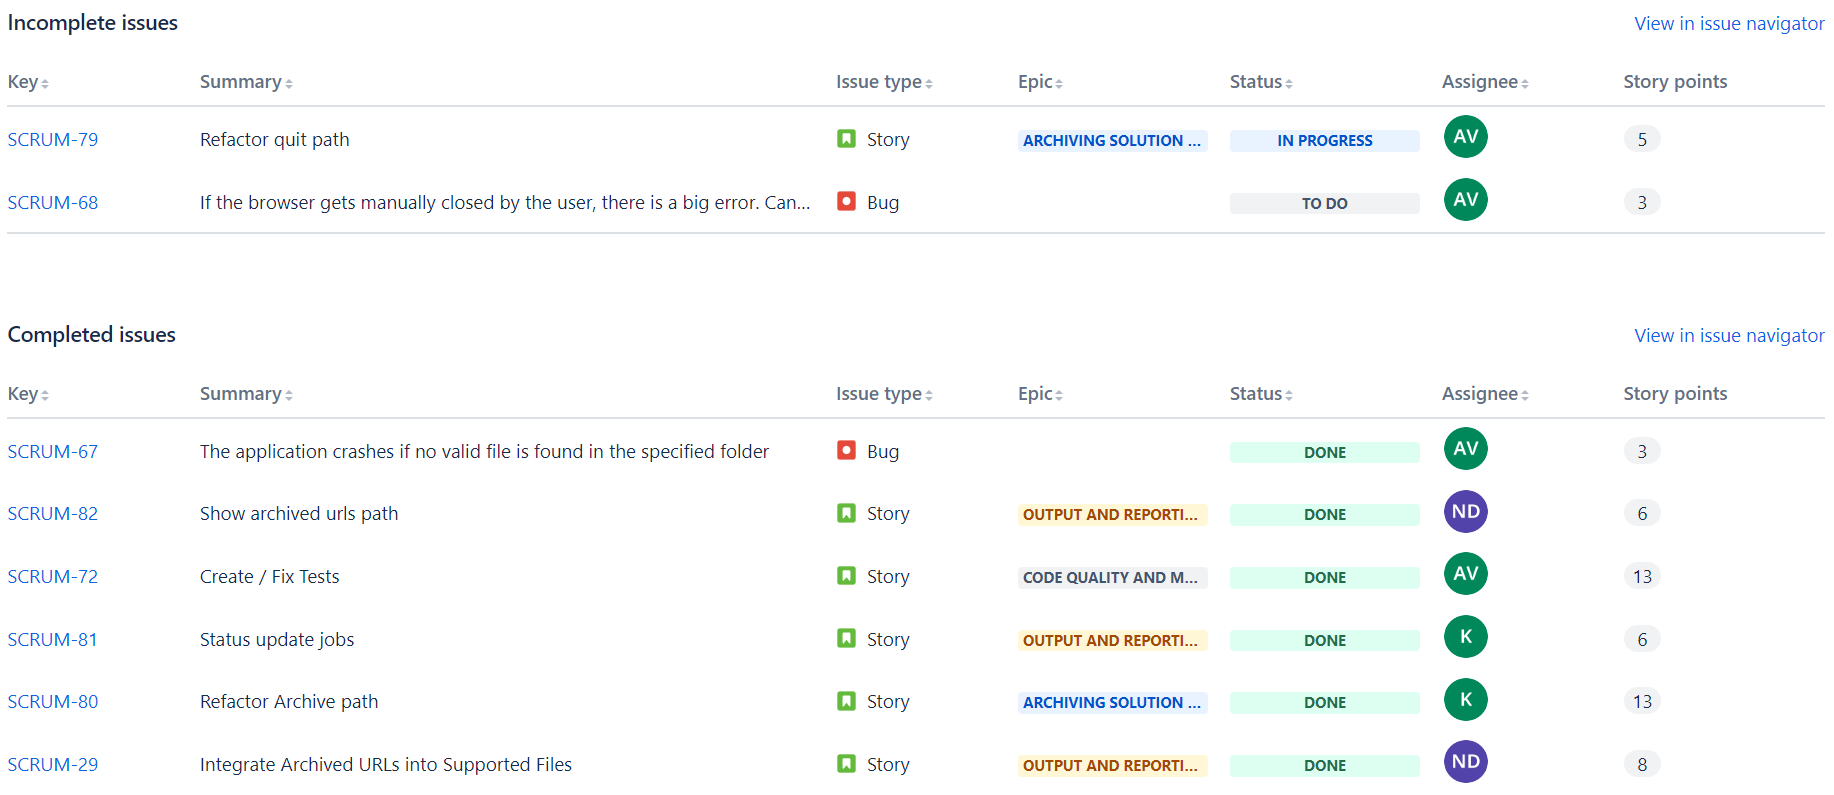
\includegraphics[width=1\textwidth]{pictures/Scrum/Sprint 5/Sprint5_Backlog}
    \caption{Sprint 5 Backlog}
    \label{fig:sprint_5_backlog}
\end{figure}

The user stories from the fifth sprint are shown below. The stories have been estimated and prioritised.
\begin{figure}[h!]
    \centering
    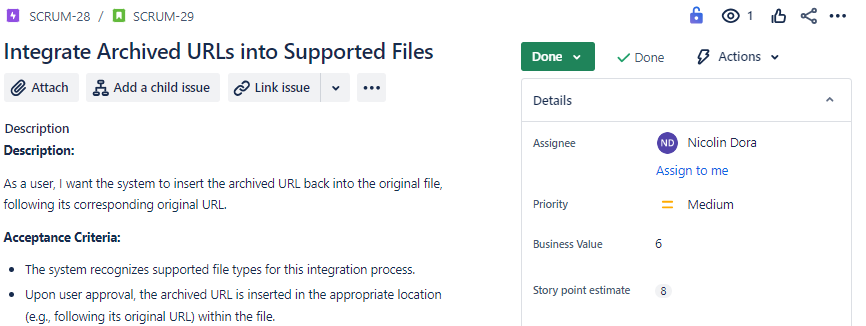
\includegraphics[width=1\textwidth]{pictures/Scrum/Sprint 5/UserStory_10}
    \caption{User Story Detail for "Integrate Archived URLs into Supported Files"}
    \label{fig:sprint_5_userstory_1}
\end{figure}
\begin{figure}[h!]
    \centering
    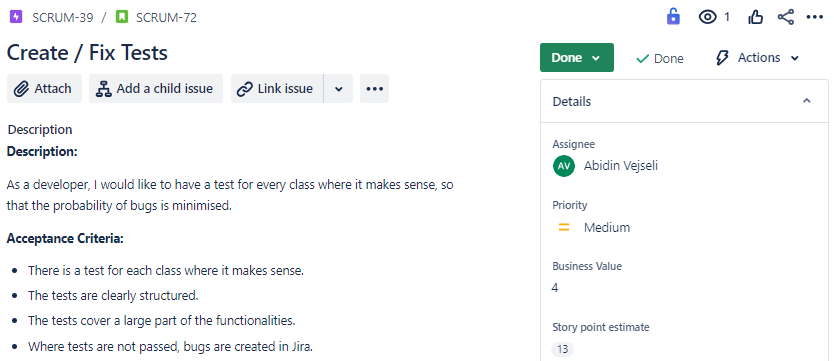
\includegraphics[width=1\textwidth]{pictures/Scrum/Sprint 5/UserStory_23}
    \caption{User Story Detail for "Create / Fix Tests"}
    \label{fig:sprint_5_userstory_2}
\end{figure}
\begin{figure}[h!]
    \centering
    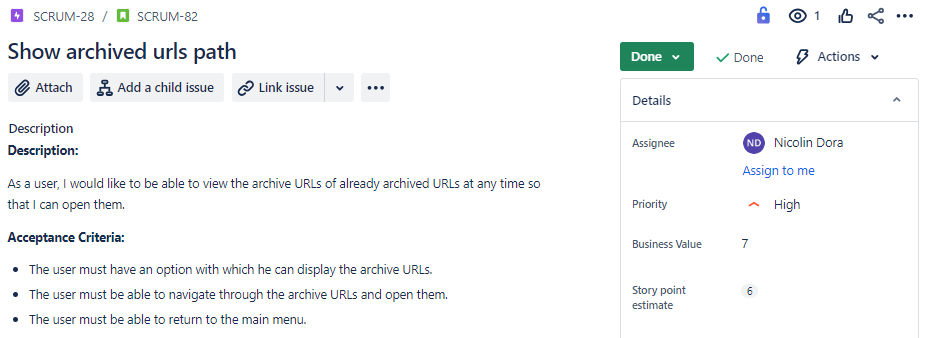
\includegraphics[width=1\textwidth]{pictures/Scrum/Sprint 5/UserStory_25}
    \caption{User Story Detail for "Show archived urls path"}
    \label{fig:sprint_5_userstory_3}
\end{figure}

In the fifth sprint, the burn down chart looks like this:
\begin{figure}[h!]
    \centering
    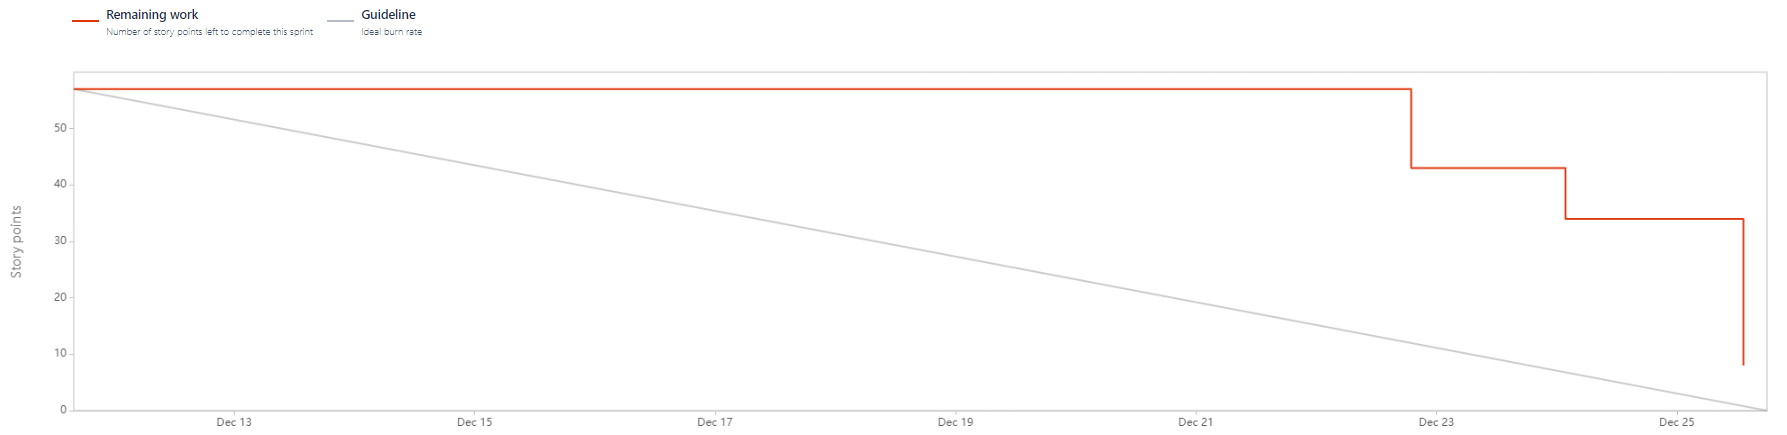
\includegraphics[width=1\textwidth]{pictures/Scrum/Sprint 5/Sprint5_Burndownchart}
    \caption{Sprint 5 Burn Down Chart}
    \label{fig:sprint_5_bunrdown_chart}
\end{figure}

In sprint 5, our time was limited due to commitments in other modules and the upcoming Christmas period, which resulted in team member absences.
We encountered an unexpected challenge with the extensive time required for test refactoring, as we prioritise quality, which often demands more time.
As a result, we were unable to complete all planned user stories and had to carry them over to the next sprint.
These challenges are reflected in the burn down chart.
\clearpage


\subsection{Scrum Adaptionen}
As part of Project 1, we have adjusted Scrum in order to use it in the best possible way. The adjustments are explained in this chapter.

\subsubsection{Definition of Ready (DOR)}
Our DOR includes conditions that ensure that all team members understand the user stories and know when a user story can be included in a sprint. The DOR was set in line with the INVEST\footnote{\href{https://xp123.com/articles/invest-in-good-stories-and-smart-tasks/}{XP123 article: Invest in good stories and smart tasks}} criteria. A user story in the product backlog must meet the DOR before it can be included in a sprint.

\textbf{Definition of Ready}
\begin{itemize}
    \item Ensure a clear definition
    \item Define the functionality or requirement to be implemented
    \item Clearly defined and testable acceptance criteria
    \item Ensure there are no or minimal dependencies
    \item Understood by the whole team
    \item The user story has been estimated
    \item The scope of the user story is small enough that it can be implemented in a single sprint.
\end{itemize}

\subsubsection{Definition of Done (DOD)}
Our DOD contains all the characteristics and standards that a user story must meet to be considered complete.
Once it satisfies the necessary quality requirements (acceptance criteria), the story can be considered complete and can be closed.
The goal of our DOD is to create transparency so that everyone has a common understanding of when a story can be closed.
A story that does not comply with the DOD may not be finalised.

\textbf{Definition of Done}
\begin{itemize}
    \item Coding standards and best practices are implemented
    \item Unit tests for the feature are written and passe
    \item Any changes to the code or functionality are documented
    \item The code and functionality are reviewed by peers
    \item The feature works across multiple platforms
    \item Code is integrated with master branch
    \item Documentation has been updated
    \item Acceptance criteria are met
\end{itemize}
\clearpage

\subsubsection{User Story Template}
For the creation of a user story, we have defined a template so that the user stories contain all the necessary information. Below is a screenshot of our template. It includes all the relevant fields for us: Assignee, Priority, Business Value, Story Points estimate and assigned Sprint. Furthermore, we describe the user story in the "Description" field in the format "AS A <user role> I WANT TO <the goal> [SO THAT <reason>]" as well as the Acceptance Criteria.
To ensure that we always have the DOR and DOD to hand, we also work with the Jira On-the-Fly add-on, which enables us to record both for each user story and tick off the individual points accordingly when they have been completed. This allows us to immediately recognise whether a user story can be included in a sprint and whether a story has been fully completed.
\begin{figure}[h!]
    \centering
    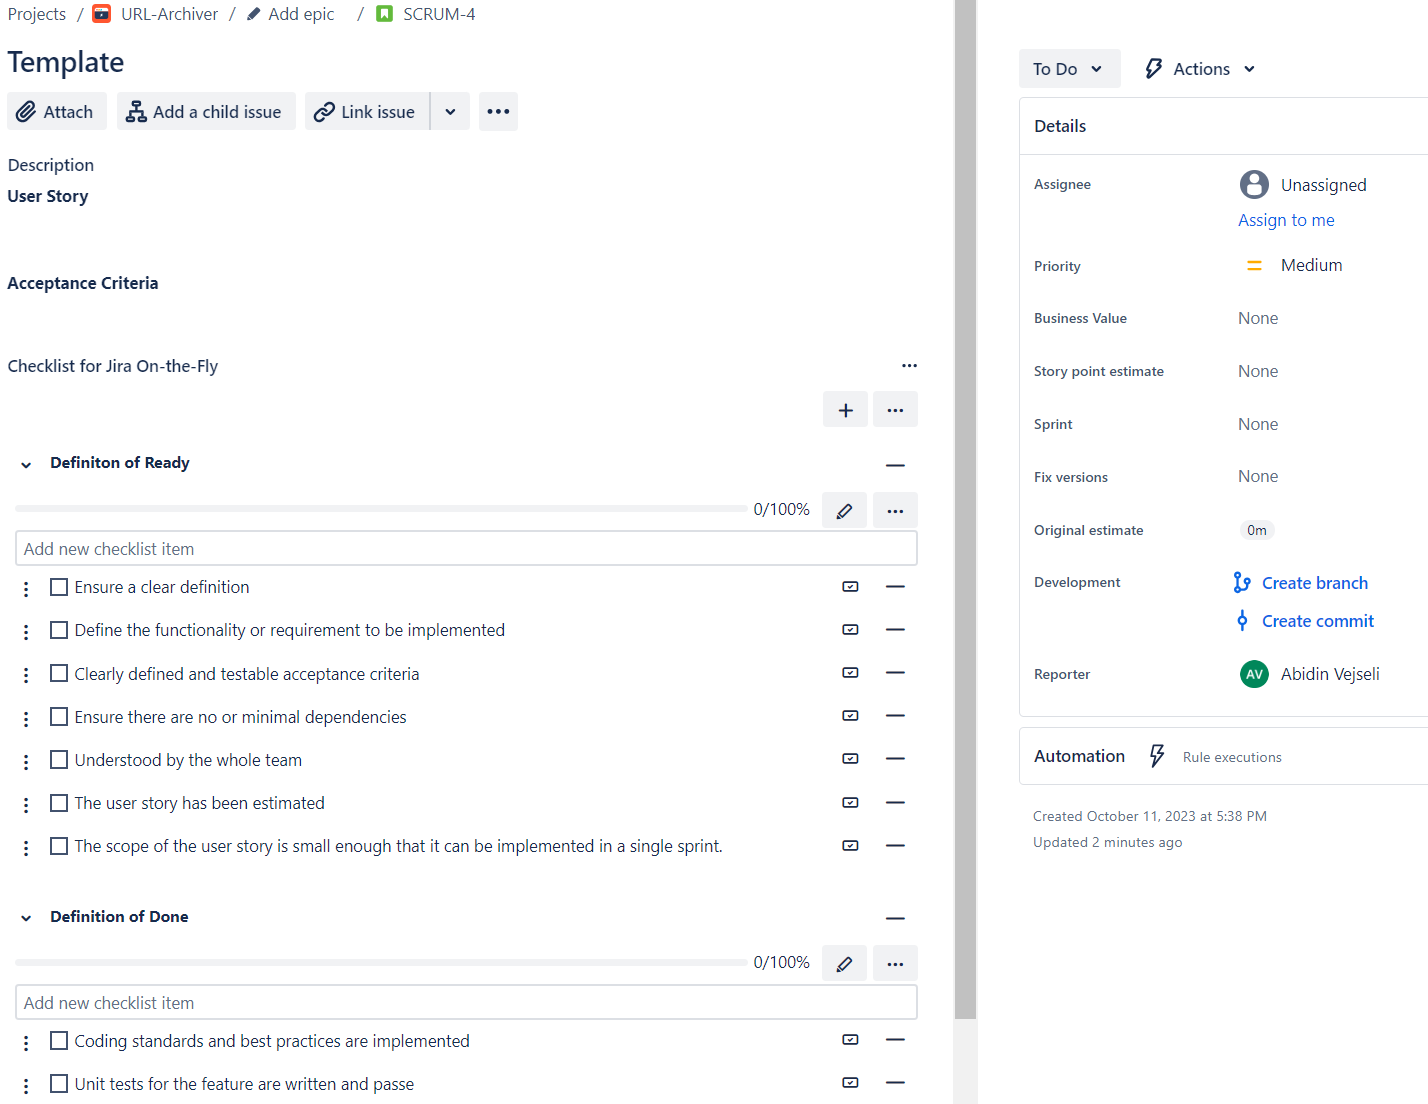
\includegraphics[width=1\textwidth]{pictures/Scrum/userstory_template}
    \caption{Screenshot from the user story template.}
    \label{fig:user_story_template}
\end{figure}
\clearpage

\subsubsection{Estimation method}
We have chosen the "T-shirt sizes" method because it is a simple way to estimate effort (story points). This method is based on the fact that everyone knows T-shirt sizes and that large sizes mean more work than small sizes. As a result, this method enables us to make efficient estimations, despite the lack of shared experience in the team.

Below is the scale we use:
\begin{figure}[h!]
    \centering
    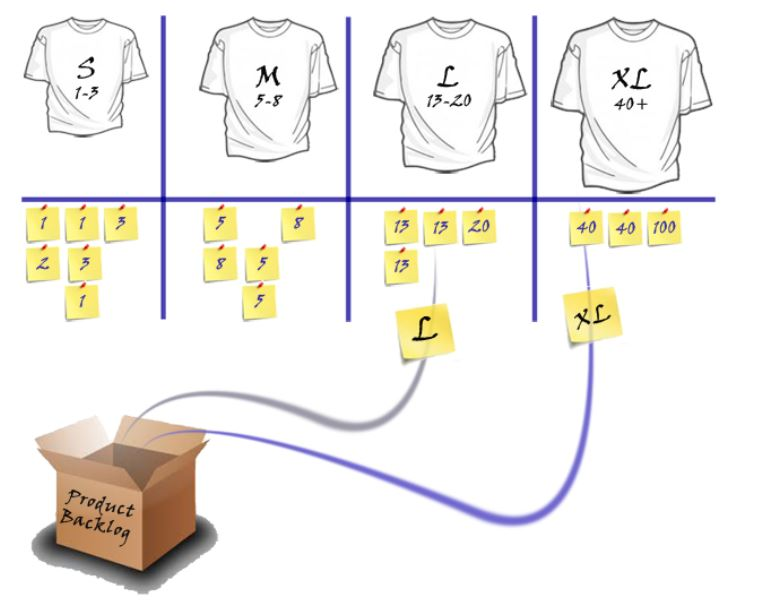
\includegraphics[width=1\textwidth]{pictures/tshirt_sizes}
    \caption{Ilustration of T-Shirt Sizes}
    \label{fig:tshirt_sizes}
\end{figure}
\clearpage

\subsubsection{Velocity}
To select the user stories and tasks to be worked on, a suitable criterion, velocity, is applied to estimate what can be completed in the upcoming sprint.

We have decided that we have a velocity of 30 story points per sprint.
Therefore, our workload per sprint should not exceed this threshold. We consciously take this into account during sprint planning.

\subsubsection{Sprint}
As a team, we have decided that our sprints will take place at two-week intervals. For each sprint we define a SMART sprint goal, which specifies the relevant user stories.

We decided in favour of the two-week rhythm because regular feedback is important to us and thus creates a greater learning effect. Additionally, we ascertained that one-week sprints would result in excessive overheads due to the administrative work involved in Scrum. Likewise, we consider sprints longer than two weeks to be impractical, as the interaction would suffer.

\subsubsection{Sprint Planning}
As part of sprint planning, we make decisions about which user stories can be implemented based on the sprint goal, the story points and the velocity.
Before a user story can be included in the sprint, it must be estimated by the Scrum team. This task is always carried out at the start of our sprint planning.
A sprint goal is then defined based on the estimated and prioritised user stories.
The user stories we select for the sprint are based on the business value, priority, story points and velocity of the team.
The sprint planning takes place on the first Monday of each sprint.
We have decided not to have a second sprint planning as we have already defined in our DOR that the user stories should be as small as possible. In addition, each developer has the opportunity to divide their user stories into tasks within the sprint. This allows a better overview of the progress in the sprint.

\subsubsection{Daily Scrum}
As a team, we have decided not to have daily Scrum meetings, as this is not possible because all team members do work part times. Instead, we have two weekly meetings (weeklys), on Wednesday and Friday at 17:00, which last a maximum of 15 minutes.
In addition, we have chosen to hold the meetings through Microsoft Teams as it is easier to organise.
The goal of these meetings is to share the current progress, address issues, update the team and briefly discuss the next steps.

\subsubsection{Sprint Review}
In the sprint review, we check the intermediate result of the processed user stories. We check whether all the stories that should be completed meet the DOD. Furthermore, we discuss in the team what went well, what problems we encountered and how we solved them. Based on these results, the product increment is created.
In our case, the product owner, who represents the customer, tests the product increment against the requirements. The review is done from the customer's perspective by testing the product increment. The outcomes are utilized to update the product backlog.
The sprint review meeting takes place on the last day of the sprint.

\subsubsection{Sprint Retrospective}
In the sprint retrospective, we gather information as a team about what went well and what didn't go as planned in the previous sprint.
We then derive specific improvements and plan their implementation. Our goal is to improve the efficiency, quality, communication and speed within our team. To achieve this, we give ourselves constructive criticism and are open to feedback.
The sprint retrospective takes place on the last day of the sprint.


%\chapter{Implementation}
%\section{Architecture}
This chapter describes the architecture of the URL-Archiver. 

\subsection{Frontend}
The frontend architecture of the URL-Archiver is centered on a console-based interface, as evidenced by the \texttt{ConsoleView} and \texttt{CLIController} classes featured in Figure \ref{fig:MVC_Highlevel}.

The \texttt{ConsoleView} class is essential for presenting information and managing user input in a console setting. It is specifically designed to display data and messages clearly and in a user-friendly way. In parallel, the \texttt{CLIController}, a key component of the Controller segment in the MVC (Model-View-Controller) framework, serves as an intermediary between the \texttt{ConsoleView} and the application’s backend. This class efficiently processes user inputs from the \texttt{ConsoleView}, liaises with the model to retrieve or alter data, and then updates the console interface with these changes. This architecture is crafted to enable streamlined and effective user interactions within a command-line environment. The Figure \ref{fig:Screenshot_ConsoleView} illustrates the welcome message that the URL archiver displays to users. 
\vskip 0.5cm
\begin{figure}[h!]
    \center
    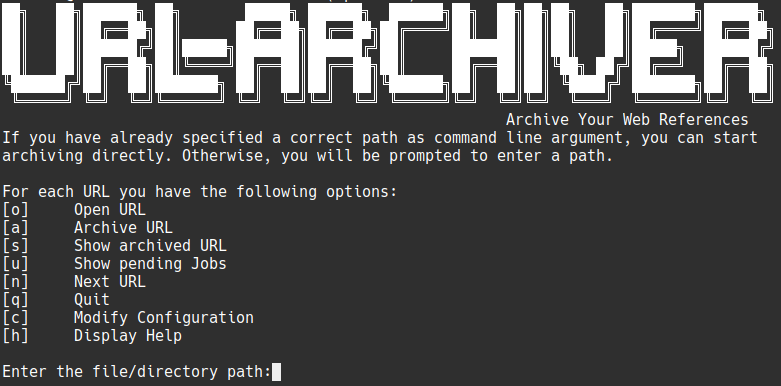
\includegraphics[width=1\textwidth]{pictures/final_presentation/command_line_application.jpg}
    \caption{Screenshot of the Console View}
    \label{fig:Screenshot_ConsoleView}
\end{figure}



\clearpage

\subsection{Backend}

\subsubsection{Software Architectural Design}
The URL-Archiver is developed following the principles of the MVC (Model-View-Controller) software architectural pattern. The MVC framework, as detailed in Figure \ref{fig:MVC_Highlevel}, is a structured approach to building user interfaces in software applications. It organizes an application into three interrelated components:

\begin{itemize}
	\item \textbf{Model:} This layer embodies the URL-Archiver's data structures, business logic, and operational rules. Components such as \texttt{FileModel}, \texttt{FolderModel}, \texttt{URLPair}, and \texttt{ConfigModel}, as shown in Figure \ref{fig:MVC_Highlevel}, represent the model.
	\item \textbf{View:} Tasked with rendering data from the model to the user and forwarding user commands to the controller. The \texttt{ConsoleView} in Figure \ref{fig:MVC_Highlevel} serves as a demonstration of this component.
	\item \textbf{Controller:} It is responsible for handling user inputs, engaging with the model to process data, and selecting the appropriate view for presentation. The \texttt{CLIController}, depicted in Figure \ref{fig:MVC_Highlevel}, is indicative of this segment.
\end{itemize}

This modular structure allows for an efficient separation of code, which aids in easier maintenance and streamlined development. The \texttt{Main} class operates as the launching point for the URL-Archiver, effectively coordinating the MVC pattern. Interaction between the Controller and the Model results in updates to the Model, with the View being refreshed in tandem to maintain a clear demarcation of responsibilities.

\begin{figure}[h!]
    \center
    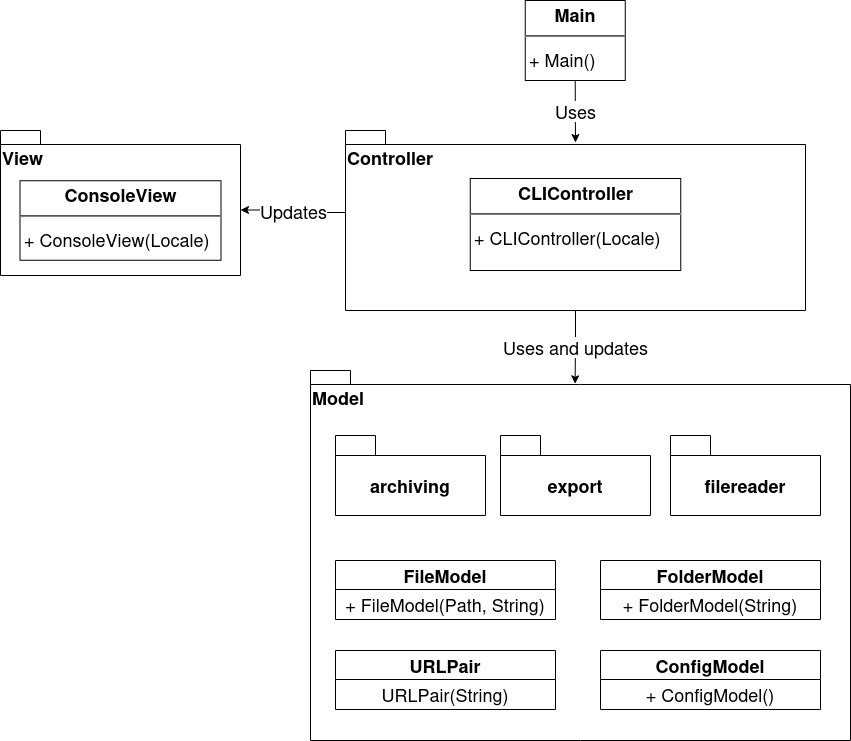
\includegraphics[width=0.7\textwidth]{diagrams/mvc_diagram-Highlevel_MVC.png}
    \caption{Highlevel Diagram of implemented MVC Pattern}
    \label{fig:MVC_Highlevel}
\end{figure}

\clearpage

\subsubsection{Factory Pattern}
The URL-Archiver makes extensive use of the Factory Pattern in its architecture, a key strategy in software engineering recognised for its role in the creational design paradigm. This pattern is central to the encapsulation of the object instantiation process. Rather than creating objects directly using the "new" operator, the Factory Pattern specifies a factory for this purpose. This abstraction improves the flexibility and scalability of the code.

The factory pattern is particularly useful when dealing with a variety of object types to be created, or when specific logic is required in their creation. Its implementation in the URL Archive provides a clear separation of concerns and improves code reusability, in line with the core principles of object-oriented design and programming.

In the URL-Archiver, the Factory Pattern is implemented in several key areas:

\begin{itemize}
	\item \textbf{File Readers:} Streamlines the addition of more input file types, thanks to its capability to produce objects conforming to the \texttt{FileReaderInterface}. This factory is pivotal in handling diverse file types.
	\item \textbf{Archiving Services:} Adding an additional service is straightforward, enhancing the application's ability to integrate different web archiving services.
	\item \textbf{Selenium Web Drivers:} Supports the integration of additional browsers with ease, showcasing the pattern’s adaptability in browser interactions.
	\item \textbf{Export Functionality:} The pattern's application here simplifies the inclusion of support for various file types in the export functionality.
\end{itemize}

These factories contribute significantly to the modularity and extensibility of the URL Archive by encapsulating the creation logic of various components, thus promoting loose coupling and scalability. The alignment of these approaches with the principles of the Factory Design Pattern underscores the maintainability of the application and its adaptability to new file types and data export formats.

The application of the factory pattern in the URL Archive is illustrated in figures \ref{fig:FileReaderFactory_Diagram} and \ref{fig:ExporterFactory_Diagram}, which show the \texttt{FileReaderFactory} and \texttt{ExporterFactory} respectively. Similar design principles are applied to other factories within the application, ensuring a consistent and modular approach across all components.

\begin{figure}[h!]
    \center
    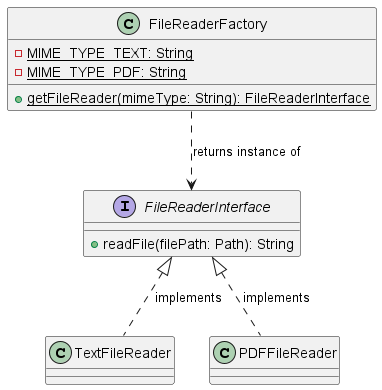
\includegraphics[width=0.5\textwidth]{pictures/FileReaderFactory-0.png}
    \caption{Diagram of the FileReader Factory}
    \label{fig:FileReaderFactory_Diagram}
\end{figure}

\begin{figure}[h!]
    \center
    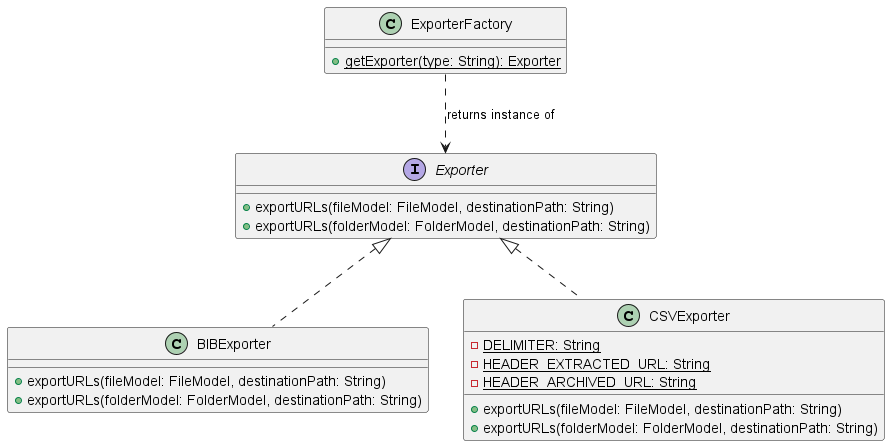
\includegraphics[width=0.9\textwidth]{pictures/ExporterFactory-0.png}
    \caption{Diagram of the Exporter Factory}
    \label{fig:ExporterFactory_Diagram}
\end{figure}

\subsubsection{Configuration File Management}
The URL-Archiver uses a JSON configuration file to effectively manage various settings and parameters. Key classes such as \texttt{ConfigModel} and \texttt{ConfigFileHelper} are integral to this process. The \texttt{ConfigModel} is used to define the structure of the configuration data, ensuring that all essential settings are systematically represented and easily accessible within the application. Conversely, the ConfigFileHelper is responsible for reading and writing the JSON configuration file, decoupling these tasks from the rest of the application code. This methodology not only streamlines the management of configuration settings, but also increases the adaptability of the application, as configuration changes do not require codebase changes.

An example of the configuration file structure is as follows:

\{

\quad''accessKey'':''[Access Key]'',

\quad''secretKey'':''[Secretkey]'',

\quad''browser'':''FIREFOX''

\}

Users have the flexibility to modify the configuration file at runtime, or edit the file directly. Currently, the application uses this file to store credentials for the Wayback Machine and to select the correct browser for the Archive Today service. This feature underlines the URL-Archiver's commitment to user customisation and operational efficiency.

\subsubsection{Adherence to SOLID Principles}
The URL-Archiver has been carefully designed with a strong emphasis on SOLID principles, ensuring a robust, maintainable and scalable architecture.

\begin{enumerate}
	\item \textbf{Single Responsibility Principle:} Each class, such as \texttt{FileReaderFactory}, \texttt{ConfigModel} or \texttt{CLIController}, is dedicated to a single responsibility. This principle ensures that each module or class focuses on a single aspect of the application's functionality.
	\item \textbf{Open/Closed Principle:} The application uses interfaces such as \texttt{FileReaderInterface} and factory classes to facilitate extensibility while keeping changes to existing code to a minimum. This approach allows new functionality to be added seamlessly.
	\item \textbf{Liskov Substitution Principle:} The architectural design allows subclasses (such as specific file readers) to replace their parent class or interface without compromising the integrity of the application, thereby maintaining a robust design.
	\item \textbf{Interface separation principle:} The design strategy of the URL Archive favours lean interfaces, ensuring that classes implement only the methods essential to their functionality. This is evident in the focused methods of interfaces such as \texttt{URLArchiver} and \texttt{Exporter}.
	\item \textbf{Dependency Inversion Principle:} High-level modules such as \texttt{CLIController} rely on abstractions rather than concrete implementations. This is emphasised by the use of interfaces and factory classes for object creation, which reduces dependency on specific implementations.
\end{enumerate}

The URL-Archiver's strict adherence to these SOLID principles is a testament to its well-structured, easily maintainable and scalable design. This approach underlines the application's commitment to high quality software engineering practices.

\subsubsection{Class Diagram}
Below the complete class diagram of this application is displayed. 

\clearpage

%\addcontentsline{lof}{figure}{UML Class Diagram URL-Archiver}
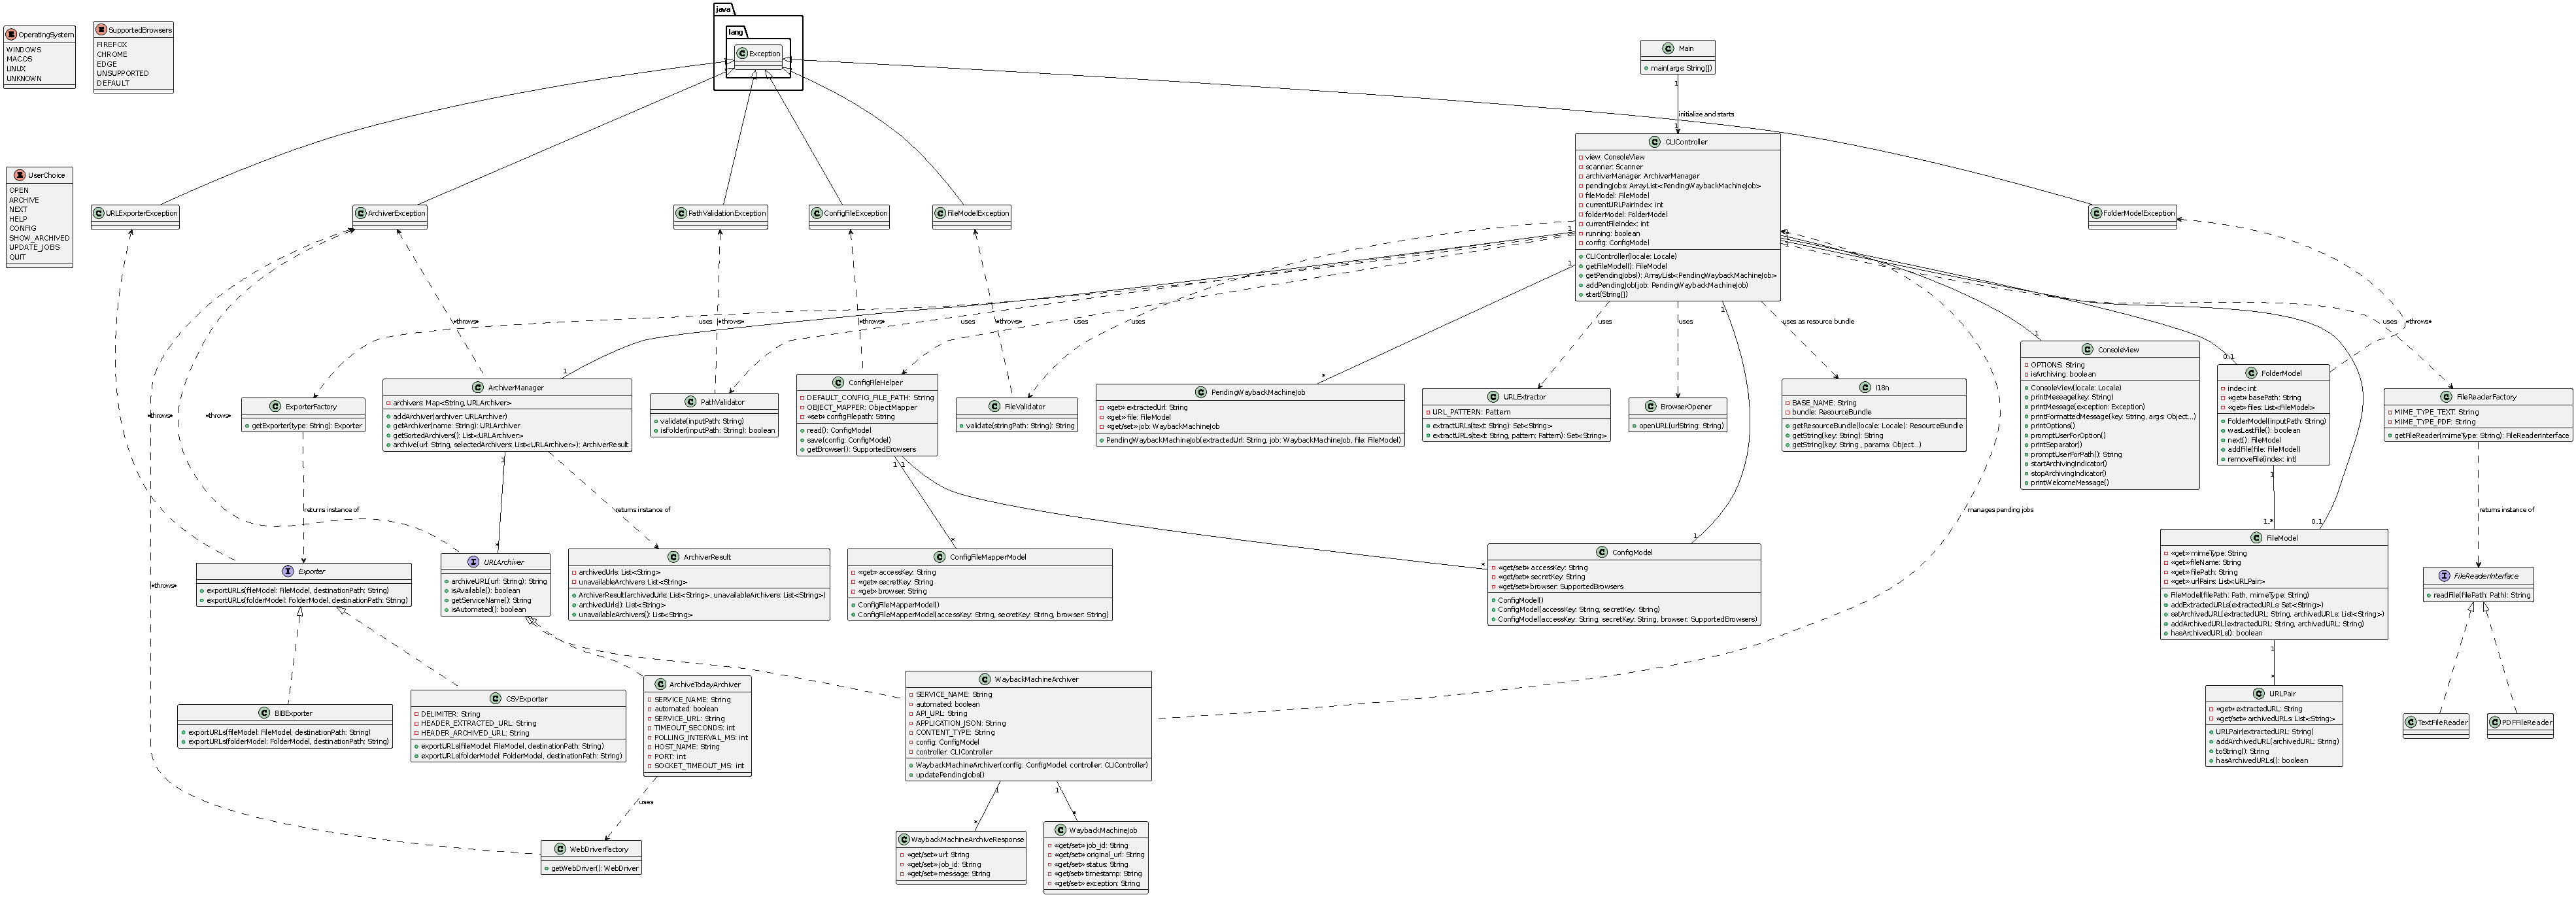
\includepdf[pages=1,fitpaper]{diagrams/uml_diagram.pdf}


%\section{Processes}
% https://www.ganttlab.com
%					https://www.hermes.admin.ch/de/projektmanagement/verstehen/ubersicht-hermes/methodenubersicht.html

\subsection{Scrum}
We implemented our project utilizing the Scrum framework.
Over the course of the project, we completed six sprints.
Within these sprints, we tackled seven Epics, and successfully completed a total of 54 User Stories.
The progression of our project, along with the milestones and deliverables achieved, is illustrated in the subsequent Gantt chart.


\subsection{Allocation of roles}
In this chapter, the Scrum roles (Product Owner, Scrum Master, Developer) and additional roles such as Customer, Stakeholder, etc. are defined.


\subsection{Scrum roles}
We have decided to structure our Scrum team in the following manner:
\begin{table}[ht]
    \centering
    \begin{bfhTabular}{lll}
        \textbf{Role} & \textbf{Person}\\\hline
        Product Owner & Nicolin Dora\\\hline
        Scrum Master  & Abidin Vejseli\\\hline
        Developer     & Nicolin Dora, Abidin Vejseli, Kilian Wampfler\\\hline
    \end{bfhTabular}
    \caption{Scrum Roles}
    \label{tab:tab1}
\end{table}

Nicolin took on the role of Product Owner as he had concrete ideas and visions for the product at the start of the project.
Additionally, he took on this role because he wanted to deal with the subjects surrounding the product backlog.

Abidin took on the role of the Scrum Master as he has the most experience with the agile way of working.
He has already had the opportunity to perform this role professionally on several smaller projects in the past.

Kilian took on the role of a Developer, as he is an active programmer in his job and has already gained some experience with Scrum.
Therefore, self-organization is not a foreign concept to him.

Besides Kilian, all the other members of the group were also assigned the role of Developer, as otherwise the project would not have been feasible in the given time. This is due to the fact that we all work alongside the university.

\subsection{Additional roles}
In addition to the Scrum roles, we have assigned the following roles to our specialist lecturer and PM-coach.
\begin{table}[ht]
    \centering
    \begin{bfhTabular}{lll}
        \textbf{Role} & \textbf{Person}\\\hline
        Stakeholder   & Dr. Simon Kramer\\\hline
        Customer      & Dr. Simon Kramer\\\hline
        PM-Advisor    & Frank Helbling\\\hline
    \end{bfhTabular}
    \caption{Additional Scrum Roles}
    \label{tab:tab2}
\end{table}

\subsection{Scrum Adaptionen}
As part of Project 1, we have adjusted Scrum in order to use it in the best possible way.
The major adjustments are explained in this chapter.

\subsubsection{Definition of Ready (DOR)}
Our DOR includes conditions that ensure that all team members understand the user stories and know when a user story can be included in a sprint. The DOR was set in line with the INVEST\footnote{\href{https://xp123.com/articles/invest-in-good-stories-and-smart-tasks/}{XP123 article: Invest in good stories and smart tasks}} criteria. A user story in the product backlog must meet the DOR before it can be included in a sprint.

\textbf{Definition of Ready}
\begin{itemize}
    \item Ensure a clear definition
    \item Define the functionality or requirement to be implemented
    \item Clearly defined and testable acceptance criteria
    \item Ensure there are no or minimal dependencies
    \item Understood by the whole team
    \item The user story has been estimated
    \item The scope of the user story is small enough that it can be implemented in a single sprint.
\end{itemize}
\clearpage

\subsubsection{Definition of Done (DOD)}
Our DOD contains all the characteristics and standards that a user story must meet to be considered complete.
Once it satisfies the necessary quality requirements (acceptance criteria), the story can be considered complete and can be closed.
The goal of our DOD is to create transparency so that everyone has a common understanding of when a story can be closed.
A story that does not comply with the DOD may not be finalised.

\textbf{Definition of Done}
\begin{itemize}
    \item Coding standards and best practices are implemented
    \item Unit tests for the feature are written and passe
    \item Any changes to the code or functionality are documented
    \item The code and functionality are reviewed by peers
    \item The feature works across multiple platforms
    \item Code is integrated with master branch
    \item Documentation has been updated
    \item Acceptance criteria are met
\end{itemize}

\subsubsection{Sprint}
As a team, we have decided that our sprints will take place at two-week intervals.
For each sprint we define a SMART sprint goal, which specifies the relevant user stories.

We decided in favour of the two-week rhythm because regular feedback is important to us and thus creates a greater learning effect.
Additionally, we ascertained that one-week sprints would result in excessive overheads due to the administrative work involved in Scrum.
Likewise, we consider sprints longer than two weeks to be impractical, as the interaction would suffer.

\subsubsection{Daily Scrum}
As a team, we have decided not to have daily Scrum meetings, as this is not possible because all team members do work part times. Instead, we have two weekly meetings (weeklys), on Wednesday and Friday at 17:00, which last a maximum of 15 minutes.
In addition, we have chosen to hold the meetings through Microsoft Teams as it is easier to organise.
The goal of these meetings is to share the current progress, address issues, update the team and briefly discuss the next steps.
%
%\chapter{Deployment/Integration}
%\LoadBFHModule{boxes}

\section{Installation (Sysadmin) Manual \& Script} \label{sec::installation_manual}
The URL archiver enables the extraction of URLs from any Unicode text or PDF file and allows for interactive archiving
on one of the supported archiving services.
\begin{bfhWarnBox}
The application was designed to be platform-independent. However, it has only been tested on the following systems, so it cannot be guaranteed to work without restrictions on other platforms.
\begin{itemize}
	\item Windows 11 (Version 23H2)
	\item Windows 10 (Version 22H2)
	\item macOS (Sonoma)
	\item Ubuntu (20.04.3 LTS)
\end{itemize}
\end{bfhWarnBox}

\subsection{Requirements}

To build and start the application, ensure that the following dependencies are installed on your system:
\begin{itemize}
	\item Git: Latest stable version recommended.
	\item Maven: Version 3.8 or higher.
	\item Java: Version 21.
\end{itemize}

\subsection{Clone the repository}

To clone the repository, run the following command in a terminal:

\begin{lstlisting}[numbers=none]
git clone https://github.com/devobern/URL-Archiver.git
\end{lstlisting}

\subsection{Build and run scripts}

The build and run scripts are provided for Windows (\texttt{build.ps1}, \texttt{run.ps1}, \texttt{build\_and\_run.ps1}), Linux, and
MacOS (\texttt{build.sh}, \texttt{run.sh}, \texttt{build\_and\_run.sh}). The scripts are located in the root directory of the project.

\begin{bfhWarnBox}
	The scripts need to be executable. To make them executable, run the following command in a terminal:
	\begin{itemize}
		\item Linux / MacOS: \texttt{chmod +x build.sh run.sh build\_and\_run.sh}
		\item Windows: 
		\begin{itemize}
			\item Open PowerShell as an Administrator. 
			\item Check the current execution policy by running: Get-ExecutionPolicy. 
			\item If the policy is Restricted, change it to RemoteSigned to allow local scripts to run. Execute: Set-ExecutionPolicy RemoteSigned. 
			\item Confirm the change when prompted.
			\item This change allows you to run PowerShell scripts that are written on your local machine. \textbf{Be sure to only run scripts from trusted sources.}
		\end{itemize}
	\end{itemize}
\end{bfhWarnBox}

\subsubsection{Windows}

\paragraph{Build the application}
\mbox{}\\
To build the application, open a command prompt and run the following script:

\begin{lstlisting}[numbers=none]
./build.ps1
\end{lstlisting}

\paragraph{Run the application}
\mbox{}\\
To run the application, open a command prompt and run the following script:

\begin{lstlisting}[numbers=none]
./run.ps1
\end{lstlisting}

\paragraph{Build and run the application}
\mbox{}\\
To build and run the application, open a command prompt and run the following script:

\begin{lstlisting}[numbers=none]
./build_and_run.ps1
\end{lstlisting}

\subsubsection{Linux and macOS}

\paragraph{Build the application}
\mbox{}\\
To build the application, open a command prompt and run the following script:

\begin{lstlisting}[numbers=none]
./build.sh
\end{lstlisting}

\paragraph{Run the application}
\mbox{}\\
To run the application, open a command prompt and run the following script:

\begin{lstlisting}[numbers=none]
./run.sh
\end{lstlisting}

\paragraph{Build and run the application}
\mbox{}\\
To build and run the application, open a command prompt and run the following script:

\begin{lstlisting}[numbers=none]
./build_and_run.sh
\end{lstlisting}


\section{User Manual}
\begin{bfhWarnBox}
	To follow the instructions in this section, the application must be built. See \ref{sec::installation_manual}.
\end{bfhWarnBox}

The URL-Archiver is a user-friendly application designed for extracting and archiving URLs from text and PDF files. Its intuitive interface requires minimal user input and ensures efficient management of URLs.

\subsection{Getting Started}

\subsubsection{Windows}

Open Command Prompt, navigate to the application's directory, and execute:

\begin{lstlisting}[numbers=none]
./run.ps1
\end{lstlisting}

\subsubsection{Linux / MacOS}

Open Terminal, navigate to the application's directory, and run:

\begin{lstlisting}[numbers=none]
./run.sh
\end{lstlisting}

\subsection{Operating Instructions}

Upon launch, provide a path to a text or PDF file, or a directory containing such files. The application will process and display URLs sequentially.

\subsubsection{Navigation}

Use the following keys to navigate through the application:

\begin{itemize}
	\item \textbf{o}: Open the current URL in the default web browser.
	\item \textbf{a}: Access the Archive Menu to archive the URL.
	\item \textbf{s}: Show a list of previously archived URLs.
	\item \textbf{u}: Update and view pending archive jobs.
	\item \textbf{n}: Navigate to the next URL.
	\item \textbf{q}: Quit the application.
	\item \textbf{c}: Change application settings.
	\item \textbf{h}: Access the Help Menu for assistance.
\end{itemize}

\subsubsection{Archiving URLs}

Choose between archiving to Wayback Machine, Archive.today, both services, or canceling.

When opting to use Archive.today for archiving, an automated browser session will initiate, requiring you to complete a captcha. Once resolved, the URL is archived, and the corresponding archived version is then collected and stored within the application.

\subsubsection{Configuration}

Customize Access/Secret Keys and the default browser. Current settings are shown with default values in brackets.

\subsubsection{Exiting}

To exit, press \textbf{q}. If a Bibtex file was provided, you'll be prompted to save the archived URLs in the Bibtex file. Otherwise, or after saving the URLs in the Bibtex file, you'll be prompted to save the archived URLs in a CSV file.

For Bibtex entries:
\begin{itemize}
	\item Without an existing note field, URLs are added as: \texttt{note = \{Archived Versions: \textbackslash url\{url1\}, \textbackslash url\{url2\}\}}
	\item With a note field, they're appended as: \texttt{note = \{<current note>, Archived Versions: \textbackslash url\{url1\}, \textbackslash url\{url2\}\}}
\end{itemize}

%\section{User Manual}
\begin{bfhWarnBox}
	To follow the instructions in this section, the application must be built. See \ref{sec::installation_manual}.
\end{bfhWarnBox}

The URL-Archiver is a user-friendly application designed for extracting and archiving URLs from text and PDF files. Its intuitive interface requires minimal user input and ensures efficient management of URLs.

\subsection{Getting Started}

\subsubsection{Windows}

Open Command Prompt, navigate to the application's directory, and execute:

\begin{lstlisting}[numbers=none, caption={Script to Run the URL-Archiver Application on Windows (User Manual)}, label={lst:user_run_win}]
	./run.ps1
\end{lstlisting}


\subsubsection{Linux / MacOS}

Open Terminal, navigate to the application's directory, and run:

\begin{lstlisting}[numbers=none, caption={Script to Run the URL-Archiver Application on Linux and macOS (User Manual)}, label={lst:user_run_unix}]
	./run.sh
\end{lstlisting}




\subsection{Operating Instructions}

Upon launch, provide a path to a text or PDF file, or a directory containing such files. The application will process and display URLs sequentially.

\subsubsection{Navigation}

Use the following keys to navigate through the application:

\begin{itemize}
	\item \textbf{o}: Open the current URL in the default web browser.
	\item \textbf{a}: Access the Archive Menu to archive the URL.
	\item \textbf{s}: Show a list of previously archived URLs.
	\item \textbf{u}: Update and view pending archive jobs.
	\item \textbf{n}: Navigate to the next URL.
	\item \textbf{q}: Quit the application.
	\item \textbf{c}: Change application settings.
	\item \textbf{h}: Access the Help Menu for assistance.
\end{itemize}

\subsubsection{Archiving URLs}

Choose between archiving to Wayback Machine, Archive.today, both services, or canceling.

When opting to use Archive.today for archiving, an automated browser session will initiate, requiring you to complete a captcha. Once resolved, the URL is archived, and the corresponding archived version is then collected and stored within the application.

\subsubsection{Configuration}

Customize Access/Secret Keys and the default browser. Current settings are shown with default values in brackets. 

To get your S3-Credentials, follow the instructions in \nameref{sub:get_cred_api}. 

\subsubsection{Exiting}

To exit, press \textbf{q}. If a BibTex file was provided, you'll be prompted to save the archived URLs in the BibTex file. Otherwise, or after saving the URLs in the BibTex file, you'll be prompted to save the archived URLs in a CSV file.

For BibTex entries:
\begin{itemize}
	\item Without an existing note field, URLs are added as: \texttt{note = \{Archived Versions: \textbackslash url\{url1\}, \textbackslash url\{url2\}\}}
	\item With a note field, they're appended as: \texttt{note = \{<current note>, Archived Versions: \textbackslash url\{url1\}, \textbackslash url\{url2\}\}}
\end{itemize}


\subsection{Getting S3-Credentials (Wayback Machine)}\label{sub:get_cred_api}

To generate your S3-Credentials, you need a Wayback Machine profile, which you can create \href{https://archive.org/account/signup}{here} (https://archive.org/account/signup).

\subsubsection{Generate S3-Credentials}
\begin{enumerate}
	\item Login to your Wayback Machine profile \href{https://archive.org/account/login}{here} (https://archive.org/account/login).
	\item Open \href{https://archive.org/account/s3.php}{this link} (https://archive.org/account/s3.php) to generate your S3-Credentials. If needed you can also delete your S3-Credentials on this page. 
\end{enumerate}
%
%\chapter{Conclusion}
%\section{Discussion}
In the course of our academic endeavor, the URL-Archiver project, we have successfully designed and implemented a Java-based application capable of extracting and archiving URLs from Unicode text and PDF documents.
This development demonstrates the practical application of our academic learning in real-world scenarios.
The application is intended to assist professionals in research and journalism by providing a streamlined approach to archive URLs and organize them.

Our project's outcome highlights the application’s proficiency in fulfilling all requirements and reaching the goal to deliver a FLOSS-licensed, platform-independent Java-program called URL-Archiver.
As young professionals in the IT field, our efforts not only gave us valuable hands-on experience, but also contributed to the larger dialogue regarding digital data management.

However, like any academic project, our application is not without its limitations.
Currently, the tool has a limited compatibility with certain file formats, which may limit its applicability.
Moreover, the necessity for manual captcha solving, while ensuring security, does pose an inconvenience and limits the tool's automation capabilities.

Looking ahead, we have a number of enhancements in mind for the URL-Archiver.
Enhancing the application's compatibility with a broader range of file formats would increase its utility.
Furthermore, integrating support for additional archiving services \index{Archiving Services}, particularly those with accessible APIs, stands as a significant upgrade.
This would not only automate interactions with a wider range of archiving solutions but also improve both the utility and user experience of the application.

In conclusion, the URL-Archiver effectively serves its intended purpose. However, there is still room for optimisation.
The findings and challenges identified during this project lay the groundwork for future improvements.
We believe that with continued research and development, the URL-Archiver can become an even more versatile and valuable tool.

%\section{Bottom Line}

\subsection{Conclusion}
The journey of developing the URL-Archiver has been a mix of unexpected challenges and rewarding experiences.
Initially assumed to be straightforward, the project revealed its complexity as we delved deeper.
This experience highlighted the importance of effective team communication, a critical factor in overcoming the unforeseen challenges of the project.
Reflecting on our approach, establishing a more robust project structure from the beginning would have been beneficial.
Despite these challenges, the project was rewarding and a great learning experience.

One of the key takeaways was the value of practical experience with Git.
This tool not only enhanced our collaborative efforts but also contributed to our personal skill development.
Remarkably, the URL-Archiver stands as our first project built entirely from scratch, marking a significant milestone in our journey as developers.

We firmly believe that the URL-Archiver has the potential to be a valuable asset to its users.
By significantly reducing the time and effort required for extracting and archiving URLs, the application promises an increase in productivity for its users.
This improvement is not just theoretical; it's a practical solution addressing a real need in the digital world.

In conclusion, while the project journey had its ups and downs, the collective learning and the potential impact of the URL-Archiver make it a fulfilling experience.
We are optimistic about its utility and look forward to seeing its adoption and evolution in the professional world.

\subsection{Productivity Increase Calculation}
This section calculates the estimated productivity increase for users of our URL-Archiver software.
The calculation factors include task duration without and with the software, the resulting time economy, cost per time unit, and overall cost economy.

\subsubsection{Assumptions}
The following assumptions were made for our calculations:
\begin{itemize}
    \item The file contains 60 URLs.
    \item Without URL-Archiver, manually finding and copying each URL takes approximately 12 seconds.
    \item The URL-Archiver takes an average of 2 seconds to find all URLs in a file.
    \item Archiving one URL using Wayback Machine manually takes 60 seconds.
    \item Archiving one URL using Archive Today manually takes 90 seconds.
    \item With URL-Archiver, initiating the archiving process for one URL in Wayback Machine takes 10 seconds. The actual archiving in the background takes in average 30 seconds.
    \item Archiving one URL using Archive Today remains at 90 seconds even with the URL-Archiver.
    \item The average hourly wage for a professional in Switzerland is CHF 40.
    \item Parallel archiving with Wayback Machine allows for multiple URLs to be archived concurrently, reducing the total time significantly.
\end{itemize}

\subsubsection{Wayback Machine Analysis}
\textbf{Without URL-Archiver:}
\begin{align*}
    \text{Task duration without SW} &= \text{URL extraction} + \text{URL archiving} \\
    &= (60 \times 12\, \text{seconds}) + (60 \times 60\, \text{seconds}) \\
    &= 720\, \text{seconds} + 3600\, \text{seconds} \\
    &= 4320\, \text{seconds (72 minutes)}
\end{align*}

\textbf{With URL-Archiver:}
\begin{align*}
    \text{Task duration with SW} &= \text{URL extraction} + \text{URL archiving} \\
    &= 2\, \text{seconds} + (60 \times 40\, \text{seconds}) \\
    &= 2\, \text{seconds} + 2400\, \text{seconds} \\
    &= 2402\, \text{seconds (40 minutes)}
\end{align*}

\textbf{Productivity Increase:}
\begin{align*}
    \text{Task duration economy} &= 72 - 40 = 32\, \text{minutes} \\
    \text{Cost per time unit} &= \frac{40\, \text{CHF}}{60\, \text{minutes}} \\
    \text{Cost economy} &= 32 \times \left( \frac{40\, \text{CHF}}{60} \right) = 21.33\, \text{CHF per document}
\end{align*}

\subsubsection{Archive Today Analysis}
\textbf{Without URL-Archiver:}
\begin{align*}
    \text{Task duration without SW} &= \text{URL extraction} + \text{URL archiving} \\
    &= (60 \times 12\, \text{seconds}) + (60 \times 90\, \text{seconds}) \\
    &= 720\, \text{seconds} + 5400\, \text{seconds} \\
    &= 6120\, \text{seconds (102 minutes)}
\end{align*}

\textbf{With URL-Archiver:}
\begin{align*}
    \text{Task duration with SW} &= \text{URL extraction} + \text{URL archiving} \\
    &= 2\, \text{seconds} + (60 \times 90\, \text{seconds}) \\
    &= 2\, \text{seconds} + 5400\, \text{seconds} \\
    &= 5402\, \text{seconds (90 minutes)}
\end{align*}

\textbf{Productivity Increase:}
\begin{align*}
    \text{Task duration economy} &= 102 - 90 = 12\, \text{minutes} \\
    \text{Cost per time unit} &= \frac{40\, \text{CHF}}{60\, \text{minutes}} \\
    \text{Cost economy} &= 12 \times \left( \frac{40\, \text{CHF}}{60} \right) = 8.00\, \text{CHF per document}
\end{align*}

%\section{Future Work}
The future vision for the URL-Archiver project includes a host of enhancements to extend its capabilities and user experience.
These potential additions, formulated within our project's limited timeframe, include:

- Adding more archiving services for a broader reach.
- Expanding support for various input file types.
- Implementing a user-friendly graphical interface.
- Enabling multilingual support for global accessibility.
- Automatically archiving all URLs in a file for efficiency.
- Providing more detailed setting options for user customization.
- Publishing the application in package repositories to simplify installation.
- Improving the code layout, like breaking up the controller for better clarity.

Integrating services such as Memento Time Travel would expand our archiving capabilities and provide a wider historical perspective.
Adapting the application to handle various file formats like .docx could increase its relevance in various other settings.
The introduction of a graphical user interface is another key area, which would dramatically improve user interaction, making the tool more accessible and engaging, particularly for those less versed in CLI environments.
Adding multilingual support is also crucial, as it would break down language barriers, enhancing the tool's usability.
The proposed enhancements, such as automatic URL archiving, detailed settings, application publishing in repositories, and code layout improvements like refactoring the controller, collectively aim to not only improve the tool's functionality and user experience but also to ensure better maintainability and ease of future extensions.


%------------ Glossary -------------------
%\printglossary

%------------ Index ----------------------
\clearpage
\printindex

%----------- Bibliography ----------------
%\clearpage
%\bibliographystyle{unsrt}
%\bibliography{project}      % the project.bib file gets loaded

%------------ Appendix ----------------	
%\appendix
%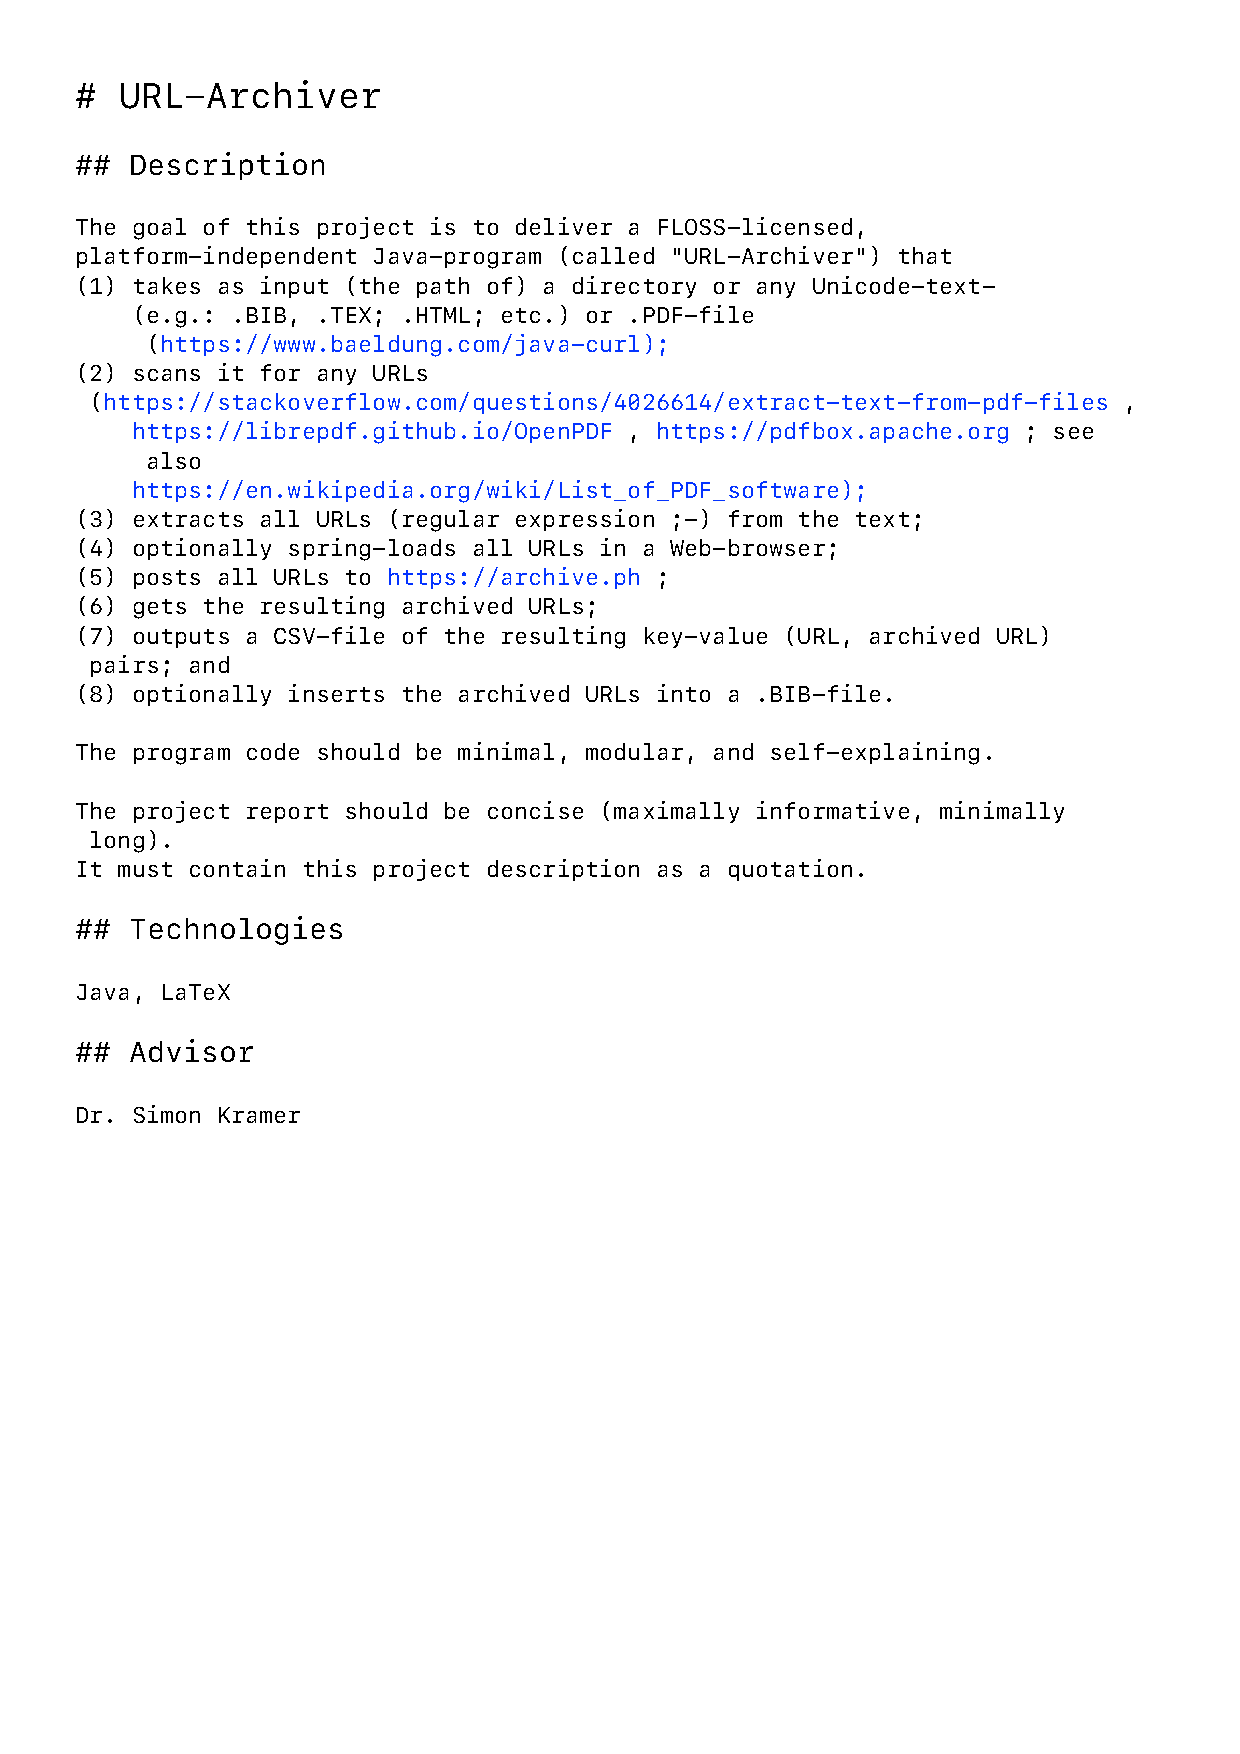
\includepdf[scale=0.9, pages=1, offset=0in -1.5in, pagecommand=\chapter{Original Project Description}]{content/kms4-03_URL-Archiver.pdf}


%------------ Authorship declaration translated to main language ------------
%\declarationOfAuthorship

\end{document}
